\chapter{Características do SMI-UnB}
\section{Visão Geral}
O SMI-UnB se baseia um sistema \textit{web} para armazenamento e coleta, setorial e temporal, dos insumos da Universidade de Brasília. Tem como base a existência de uma administração central e prédios contidos nos \textit{campi} da UnB. A administração central é expressa por um servidor mestre e realiza a gerência de todo o sistema, ou seja, todos os prédios, usuários e afins são cadastrados nela. Os prédios dos \textit{campi} são representados por servidores escravos e são responsáveis por coletar e armazenar seus insumos consumidos. O insumo escolhido para monitoramento, em um primeiro momento, foi o de energia.

De tempos em tempos, o servidor mestre realiza uma sincronização de informações com todos os servidores escravos, objetivando unificar os insumos da Universidade na administração central.

\section{Tecnologias Escolhidas}
Definiu-se a utilização do \textit{framework} Django \cite{django_project} como estrutura base do SMI-UnB, visto que o sistema consistiria em uma aplicação \textit{web} e não haveria nenhuma limitação que impedisse a utilização desse.

    \subsection{Django}
    O Django é um \textit{framework} para desenvolvimento \textit{web} implementado na linguagem Python\footnote{\url{https://www.python.org/}}. Sua arquitetura se inspira no modelo tradicional MVC (\textit{Model} \textit{View} \textit{Controller}), porém, com algumas especificidades. A comunidade \textit{Django} adota o acrônimo MTV (\textit{Model} \textit{Template} \textit{View}), onde os papéis de \textit{model}, \textit{view} e \textit{controller} são redefinidos como:
    \begin{itemize}
        \item \textit{Model}: corresponde à \textit{model} do MVC tradicional e representa as classes que popularão as tabelas do banco de dados. O \textit{Django} possui um \textit{Object-Relational Mapping} (ORM), para realizar a manipulação dessas tabelas, não sendo necessária a escrita de consultas em SQL para a persistência das informações;
        \item \textit{Template}: corresponde aproximadamente à \textit{view} do MVC tradicional e descreve como as informações serão apresentadas para o usuário;
        \item \textit{View}: representada por uma função \textit{callback} referente a uma classe de URLs, descrevendo quais informações serão apresentadas e como elas serão enviadas para o \textit{template}. Alguns autores defendem que a view corresponde ao \textit{controller} do MVC tradicional, mas para os próprios desenvolvedores do \textit{Django}, a \textit{view} deve ser minimalista e boa parte do papel do \textit{controller} deve ser implementado nas próprias classes dos modelos.
    \end{itemize}

    Na nomenclatura do \textit{Django}, um conjunto de funcionalidades pode ser agrupado em uma aplicação, chamada de \textit{app}. Cada aplicação possui suas próprias \textit{models}, \textit{views} e \textit{templates}.

    A Figura \ref{django-arq} mostra a arquitetura do \textit{Django}, apresentando as camadas do MTV durante a comunicação com o navegador até o acesso ao banco de dados. O \textit{URL dispatcher} identifica endereços requisitados pelo usuário e realiza o redirecionamento da requisição para a aplicação correta. A coordenação de requisições entre o \textit{URL dispatcher} e a \textit{view} e da \textit{view} até o \textit{template} é feita pelos chamados \textit{Middlewares}. Os \textit{Middlewares} realizam a persistência de informações entre as diferentes camadas.

    \begin{figure}[h]
        \centering
        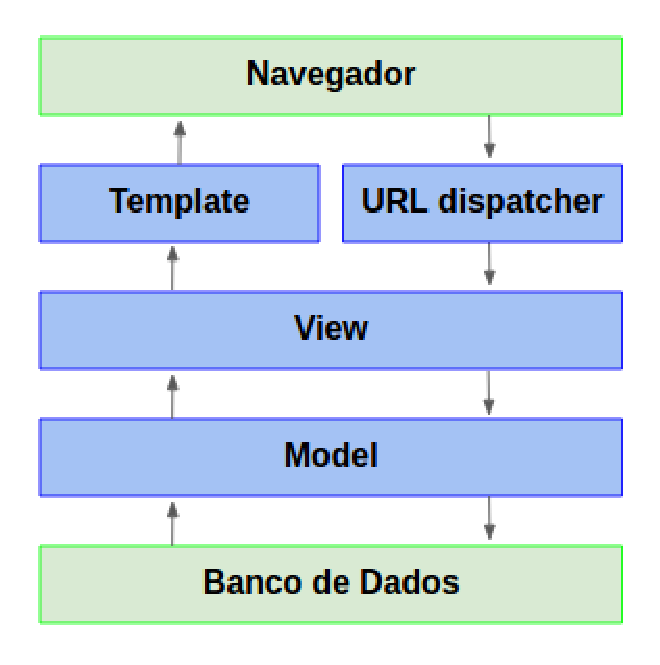
\includegraphics[keepaspectratio=true,scale=0.5]{figuras/django-arquitetura.eps}
        \caption{Arquitetura MTV \textit{Django}.}
        \label{django-arq}
    \end{figure}

\section{Protocolos Utilizados}
Antes de começar o desenvolvimento, foi necessário realizar um profundo estudo sobre o equipamento para medição de dados de energia, comumente chamado de transdutor, visto que esse já havia sido pré-designado para utilização, devido a contratos realizados anteriormente pela Universidade de Brasília.

O equipamento em questão foi o TR 4020, Figura \ref{tr4020}, disponibilizado pela empresa Embrasul \cite{embrasul}. Segundo seu manual, possui período de amostragem a cada 50 ms, comunica-se utilizando o protocolo de comunicação Modbus, no modo RTU, com velocidades de 10M/100Mbps em sistemas Ethernet, utilizando o protocolo UDP como transporte. No datagrama UDP, no campo de dados, o protocolo ModBUs-RTU é encapsulado, sendo que a porta de comunicação padrão é a 1001. O endereço ModBus dos equipamentos por padrão é 1, onde a diferenciação entre equipamentos se dá pelo número de IP.

\begin{figure}[!h]
    \centering
    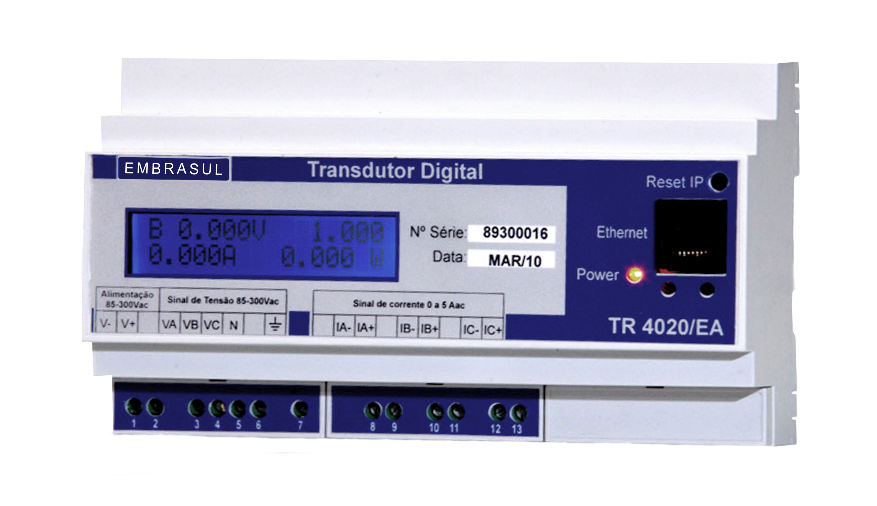
\includegraphics[keepaspectratio=true,scale=0.5]{figuras/tr4020.eps}
    \caption{Transdutor TR4020. Fonte: \cite{embrasul}}
    \label{tr4020}
\end{figure}

    \subsection{\textit{Modbus-RTU}}

    \textit{Modbus} \cite{modbus} é um protocolo serial utilizado para transmitir informações entre dispositivos eletrônicos. Suas mensagens utilizam a arquitetura de mestre-escravo, como mostra a Figura \ref{mestre_escravo}. Nesta arquitetura, o papel de mestre é designado ao dispositivo que envia as requisições e de escravo ao que responde passivamente a elas.

    \begin{figure}[!htb]
        \centering
        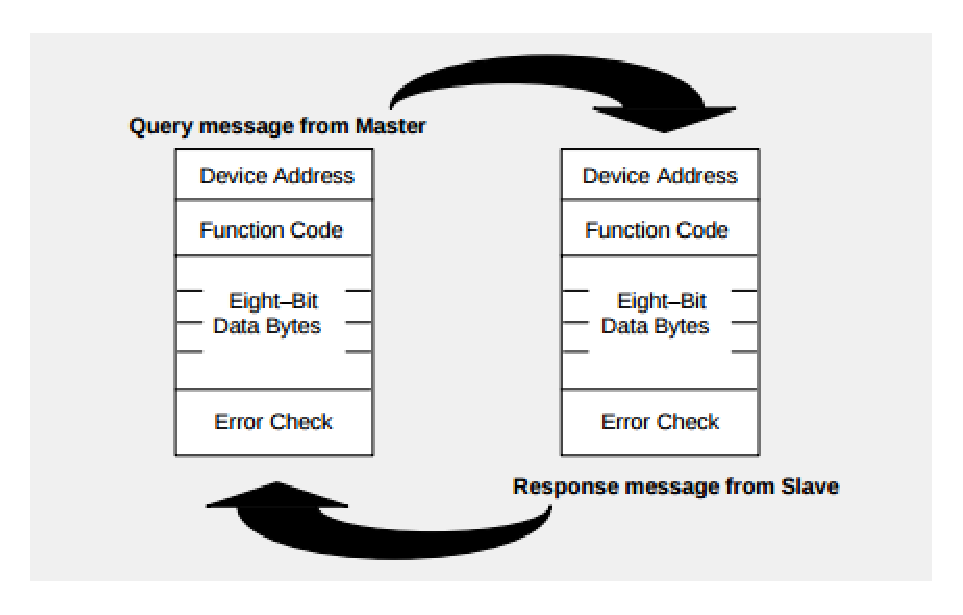
\includegraphics[keepaspectratio=true,scale=0.8]{figuras/mestre_escravo.eps}
        \caption{Comunicação Mestre-Escravo \textit{Modbus}. Fonte: \cite{modbus}}
        \label{mestre_escravo}
    \end{figure}

    Quando controladores são configurados para se comunicarem em uma rede Modbus, usando o modo \textit{Remote Terminal Unit} (RTU), cada \textit{byte} contem duplas hexadecimais de 4 \textit{bits}. A maior vantagem em se utilizar esse modo é que sua grande densidade de caracteres permite uma maior taxa de transferência comparado ao modo ASCII, em uma mesma taxa de transmissão \cite{modbus}.

    Uma mensagem em Modbus RTU possui 16 \textit{bytes} e é definida da seguinte maneira:
    \begin{itemize}
        \item Identificador do Aparelho: 2 \textit{bytes};
        \item Código de Função: 2 \textit{bytes}, define qual tipo de operação o equipamento irá realizar;
        \item Campo de Dados: 8 \textit{bytes}, sendo 4 \textit{bytes} para indicar o endereço do primeiro registrador requisitado e 4 \textit{bytes} para indicar a quantidade de registradores que serão lidos;
        \item \textit{Cyclic Redundancy Check} (CRC): 4 \textit{bytes} para verificação de erros.
    \end{itemize}

    A resposta do escravo possui a seguinte estrutura:

    \begin{itemize}
        \item Identificador do Aparelho: 2 \textit{bytes};
        \item Código de Função: 2 \textit{bytes}, define qual tipo de operação o equipamento irá realizar;
        \item Tamanho do \textit{Payload}: 2 \textit{bytes}, define o tamanho do campo de dados em \textit{bytes};
        \item Campo de Dados: possui tamanho variável, de acordo com o valor do campo anterior;
        \item \textit{Cyclic Redundancy Check} (CRC): 4 \textit{bytes} para verificação de erros.
    \end{itemize}

    \subsubsection{Leitura utilizando equipamento TR4020}
    O transdutor TR4020 possui valores em inteiro ou ponto flutuante para os registros armazenados em seus registradores. Para ler e compor um valor em inteiro, deve-se realizar a leitura de 1 registro Modbus (16 \textit{bits}), sendo que esse registro possui 2 \textit{bytes} concatenados em sequência como \textit{Byte}-A e \textit{Byte}-B, sendo o \textit{Byte}-A mais significativo. Para valores em ponto flutuante \cite{ieee754}, é realizada a leitura de 2 registros Modbus (16 \textit{bits} cada). Esse registro possui 4 \textit{bytes} concatenados em sequência como \textit{Byte}-A, \textit{Byte}-B, \textit{Byte}-C e \textit{Byte}-D. Por exemplo, para ler um valor em ponto flutuante que expressa a tensão na fase A (endereços 68 e 69), escreve-se na comunicação a sequência de \textit{bytes}, conforme a Figura \ref{request_tr4020}.

    \begin{figure}[!h]
        \centering
        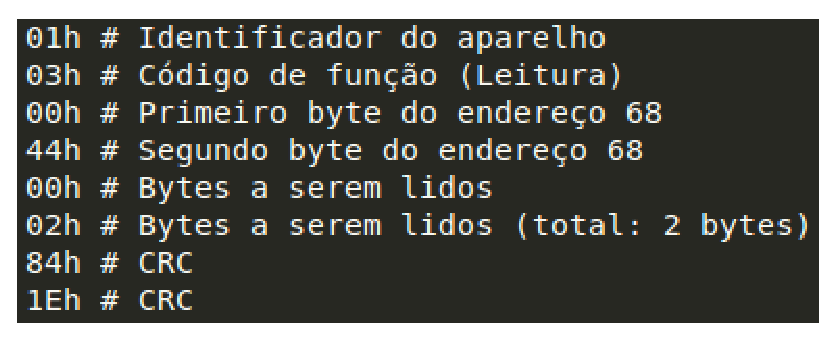
\includegraphics[keepaspectratio=true,scale=0.8]{figuras/request_tr4020.eps}
        \caption{Requisição para leitura de tensão na fase A, utilizando TR4020.}
        \label{request_tr4020}
    \end{figure}

    Tem-se como resultado, por exemplo, a resposta contida na Figura \ref{request_tr4020}.

    \begin{figure}[!h]
        \centering
        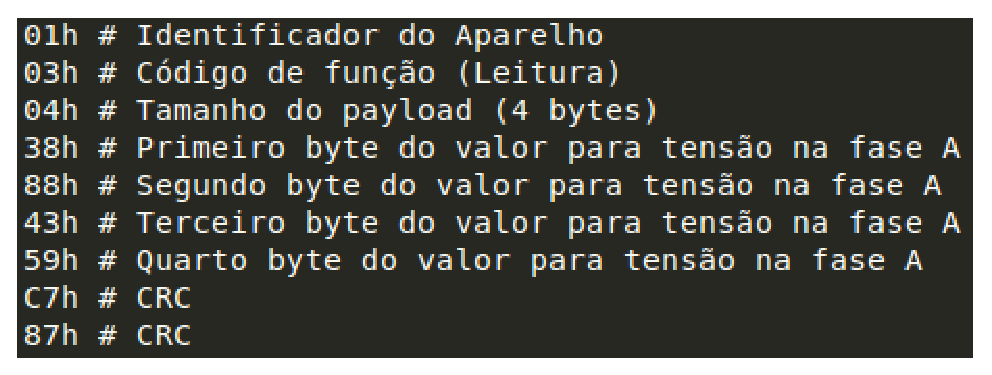
\includegraphics[keepaspectratio=true,scale=0.8]{figuras/response_tr4020.eps}
        \caption{Resposta para leitura de tensão na fase A, utilizando TR4020. O exemplo representa um valor de 217.220 para a leitura da tensão.}
        \label{request_tr4020}
    \end{figure}

    O procolo utiliza o padrão \textit{big endian} \cite{tanenbaum_1998} para representação de números inteiros, enquanto a maioria das máquinas atualmente utiliza o padrão \textit{little endian}, assim, é necessário inverter a ordem dos \textit{bytes} para transmitir os valores de tensão. O padrão \textit{little endian} define que a organização dos \textit{bytes} de uma palavra deve começar dos \textit{bits} menos significativos para os mais significativos, enquanto o \textit{big endian} utiliza a ordem reversa.

    \subsection{UDP}
    O protocolo \textit{User Datagram Protocol} (UDP) é um protocolo da camada de transporte, não orientado a conexões. Seu cabeçalho, Figura \ref{udp_header}, possui 8 \textit{bytes}, seguido de uma carga útil. As portas apresentadas no cabeçalho representam as máquinas de origem e destino \cite{tanenbaum_2002}.

    \begin{figure}[!htpb]
        \centering
        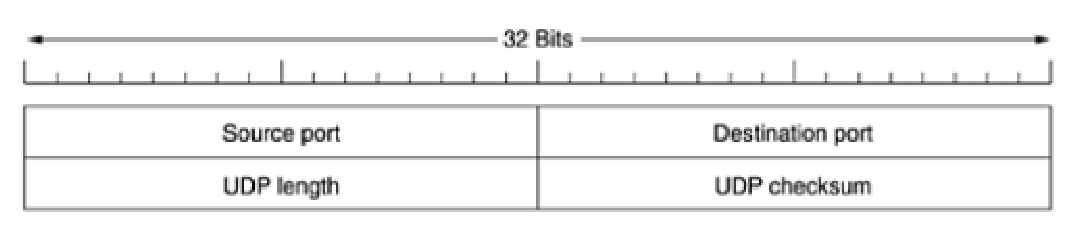
\includegraphics[keepaspectratio=true,scale=0.8]{figuras/udp_header.eps}
        \caption{Cabeçalho do UDP. Fonte: \cite{tanenbaum_2002}}
        \label{udp_header}
    \end{figure}

    Para Tanenbaum, a camada de transporte é o núcleo de toda a hierarquia de protocolos. Sua função é promover uma transferência de dados confiável e econômica entre a máquina de origem e a máquina de destino, independente das redes físicas em uso no momento.

    Nas redes de acesso empresarial, uma rede de área local (LAN) é usada para conectar um sistema final a um roteador de borda. Existem muitos tipos diferentes de tecnologias LAN. No entanto, a \textit{Ethernet} é a tecnologia de acesso mais prevalente nas redes corporativas. A \textit{Ethernet} opera 10 Mbps ou 100Mbps e utiliza cabos par trançado para conectar uma série de sistemas finais uns com os outros e com um roteador de borda. O roteador de borda é responsável por rotear pacotes que tenham destinos fora dessa LAN. A \textit{Ethernet} usa um meio compartilhado para que os usuários finais compartilhem a taxa de transmissão da LAN \cite{kurose_2002}.

    O protocolo de camada de rede da Internet se chama ``Protocolo da Internet'', ou IP. O IP fornece comunicação lógica entre hosts, possuindo um modelo de entrega de melhor esforço. Isso significa que o IP realiza seu ``melhor esforço'' para fornecer segmentos entre hosts comunicantes, mas não oferece garantias. Em particular, não garante a entrega do segmento, não garante a entrega ordenada de segmentos e garante a integridade dos dados nos segmentos \cite{kurose_2002}.

\section{Armazenamento das Informações}
Definiu-se que os \textit{campi} da UnB seriam divididos por região administrativa, cada campus teria um conjunto de edifícios, cada edifício poderia possuir diversos transdutores e os transdutores realizariam diversas medições. Para que isso fosse possível, criou-se os \textit{apps} \textit{campuses}, \textit{buildings} e \textit{transductor}.

A ferramenta utilizada para realizar os diagramas de classes dos \textit{apps} do SMI-UnB foi a StarUML\footnote{\url{http://staruml.io/}}. Além disso, não foram expressas nos diagramas as classes referentes as \textit{views} e formulários (\textit{forms}), objetivando uma menor poluição visual.

No \textit{app} \textit{campuses}, Figura \ref{campuses}, são definidos os modelos para uma região administrativa e os \textit{campi} em si.

\begin{figure}[!h]
    \centering
    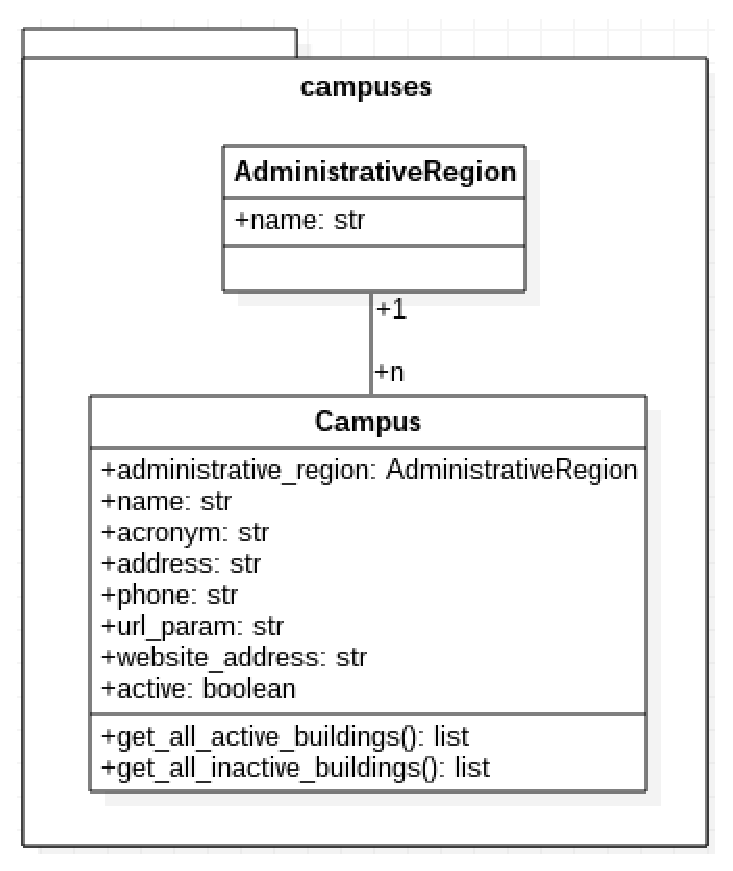
\includegraphics[keepaspectratio=true,scale=0.8]{figuras/campuses.eps}
    \caption{Diagrama de Classes para \textit{app} \textit{campuses}.}
    \label{campuses}
\end{figure}

Seguindo o mesmo princípio, o \textit{app} \textit{buildings}, Figura \ref{buildings}, define um modelo para os edifícios e possui um \textit{manager}, buscando auxiliar a manipulação de seus \textit{querysets}. Um \textit{queryset} representa uma coleção de objetos do banco de dados \cite{django_project}.

\begin{figure}[!h]
    \centering
    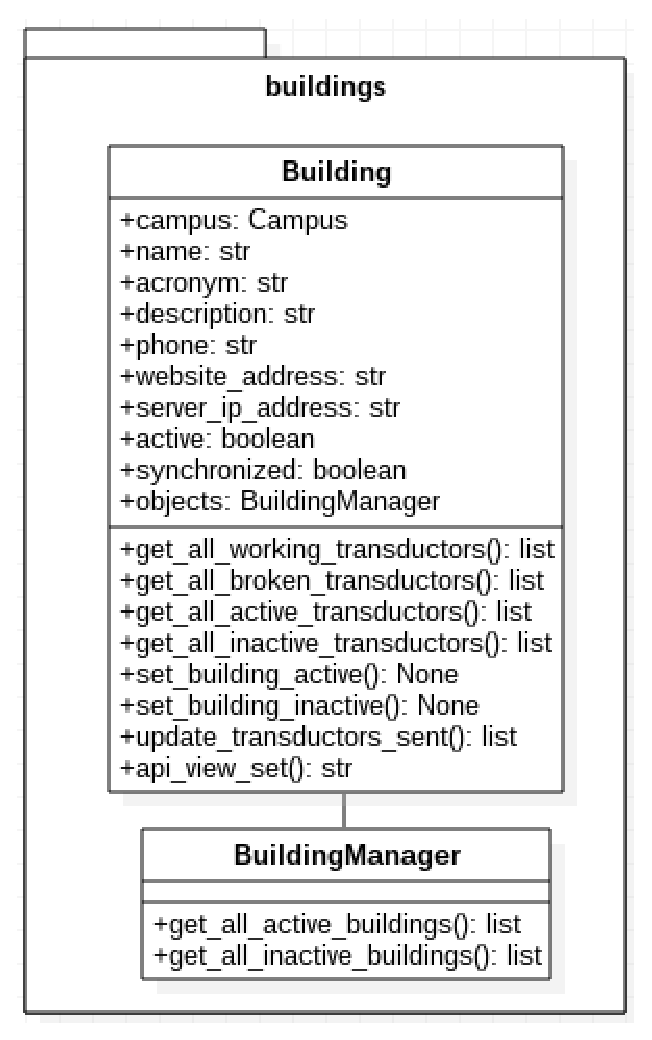
\includegraphics[keepaspectratio=true,scale=0.8]{figuras/buildings.eps}
    \caption{Diagrama de Classes para \textit{app} \textit{buildings}.}
    \label{buildings}
\end{figure}

As medições de energia iriam seguir o esquema de um sistema trifásico, onde suas fases foram representadas como A, B e C. Os parâmetros afetos ao suprimento de energia elétrica
definidos para serem coletados foram:

\begin{itemize}
    \item Tensão;
    \item Corrente;
    \item Potência Ativa;
    \item Potência Reativa;
    \item Potência Aparente.
\end{itemize}

Os transdutores e suas medições são definidos no \textit{app} \textit{transductor}, Figura \ref{transductor}. Uma das peculariedades presente nos transdutores é a necessidade de um modelo de transdutor. Esses modelos, definidos pela classe \textit{TransductorModel}, possuem toda a informação necessária para que seja possível realizar a coleta de dados, definindo o endereço e o tipo (\textit{int} ou \textit{float}) dos registradores que serão lidos, além dos protocolos seriais e de transporte utilizados.

\begin{figure}[!h]
    \centering
    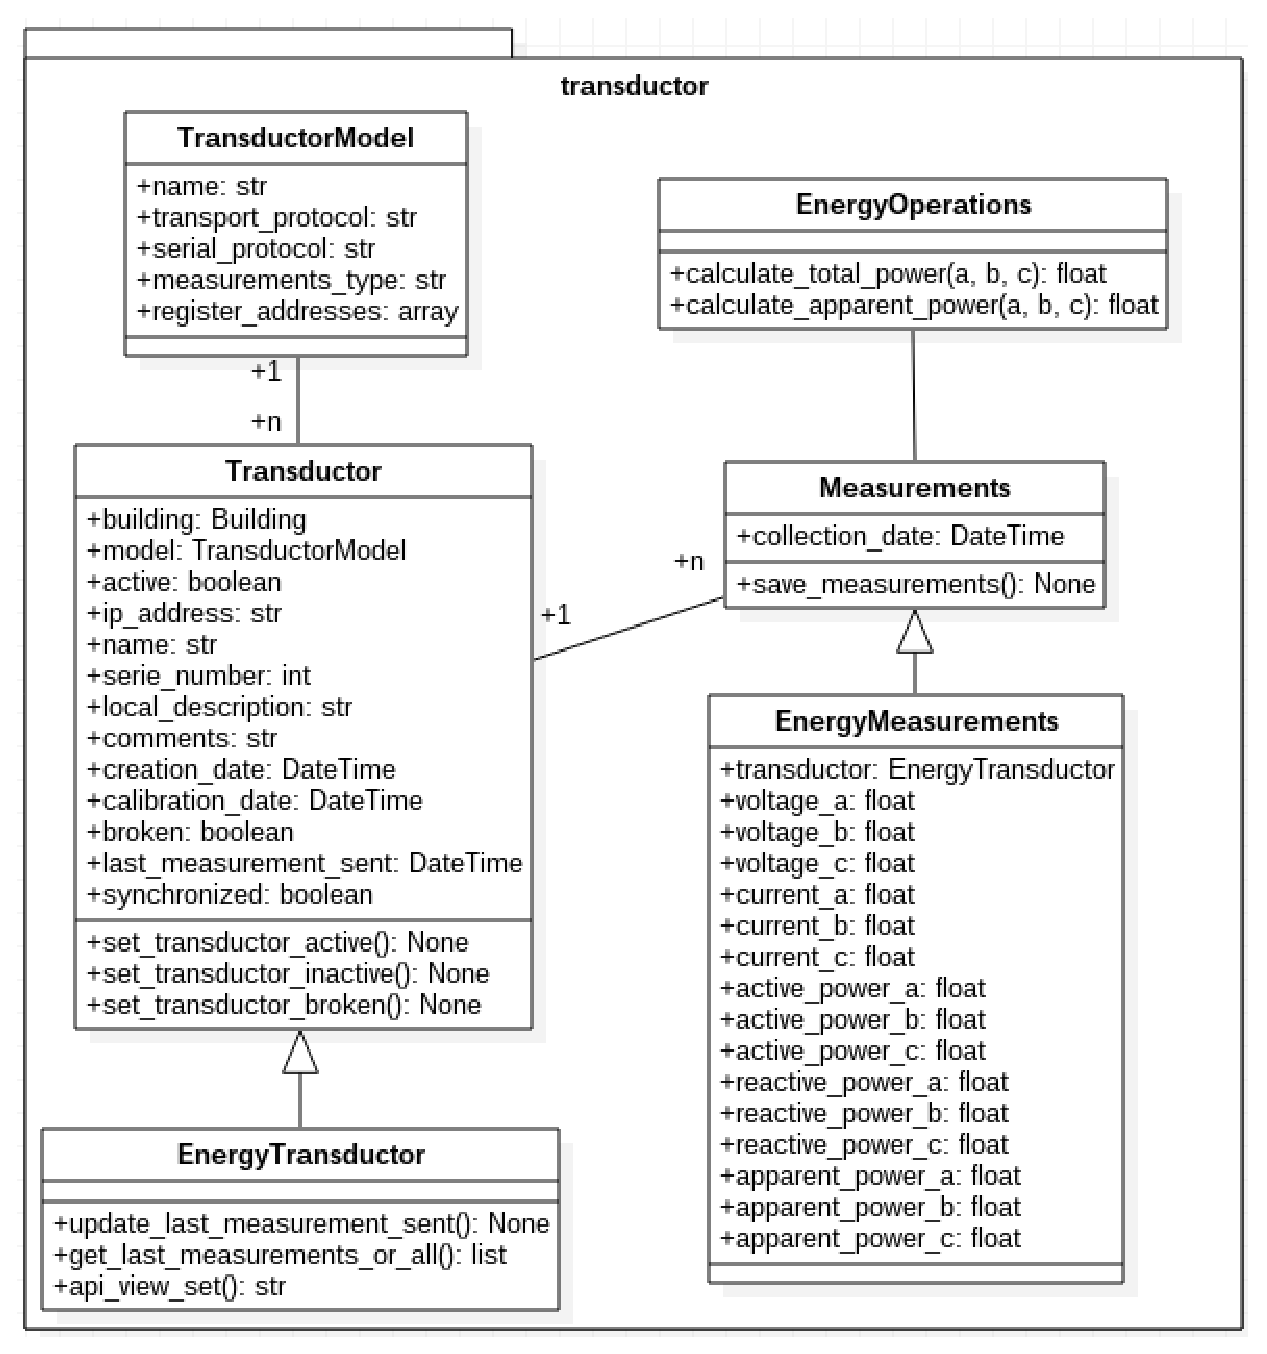
\includegraphics[keepaspectratio=true,scale=0.7]{figuras/transductor.eps}
    \caption{Diagrama de Classes para \textit{app} \textit{transductor}.}
    \label{transductor}
\end{figure}

As classes \textit{Transductor} e \textit{Measurements} são \textit{Polymorphic Models}\footnote{\url{https://django-polymorphic.readthedocs.io/en/stable/}} e possuem alguns métodos base. Com essas classes é possível extrair com mais facilidade e rapidez todas as suas classes filhas, que no caso seriam as representações dos recursos monitorados pela UnB. As especializações criadas foram referentes aos transdutores de energia e medições de energia, representados pelas classes \textit{EnergyTransductor} e \textit{Energymeasurements}. Além disso, existe uma classe auxiliar, chamada \textit{EnergyOperations}, responsável por realizar cálculos matemáticos com os dados de energia coletados.

\section{Coleta de dados}
Definiu-se que existirão dois tipos de servidores para ser possível realizar a coleta de dados inter-campi: mestre e escravo. O servidor mestre seria a representação da administração central e os escravos seriam prédios, espalhados pelos \textit{campi} da UnB, que realizariam a coleta de dados de seus transdutores, presentes na sua mesma rede.

O tempo para coleta das informações foi definido da seguinte maneira:

\begin{itemize}
    \item A cada 1 hora, o servidor mestre seria responsável por realizar uma sincronia com todas as medições realizadas pelos escravos;
    \item A cada 1 minuto, os servidores escravos seriam responsáveis por realizarem suas coletas de dados.
\end{itemize}

\subsection{Servidor Escravo}
A coleta de dados, realizada por um prédio (servidor escravo), é feita com o auxílio do app \textit{data\_reader}, Figura \ref{data_reader}.

\begin{figure}[!h]
    \centering
    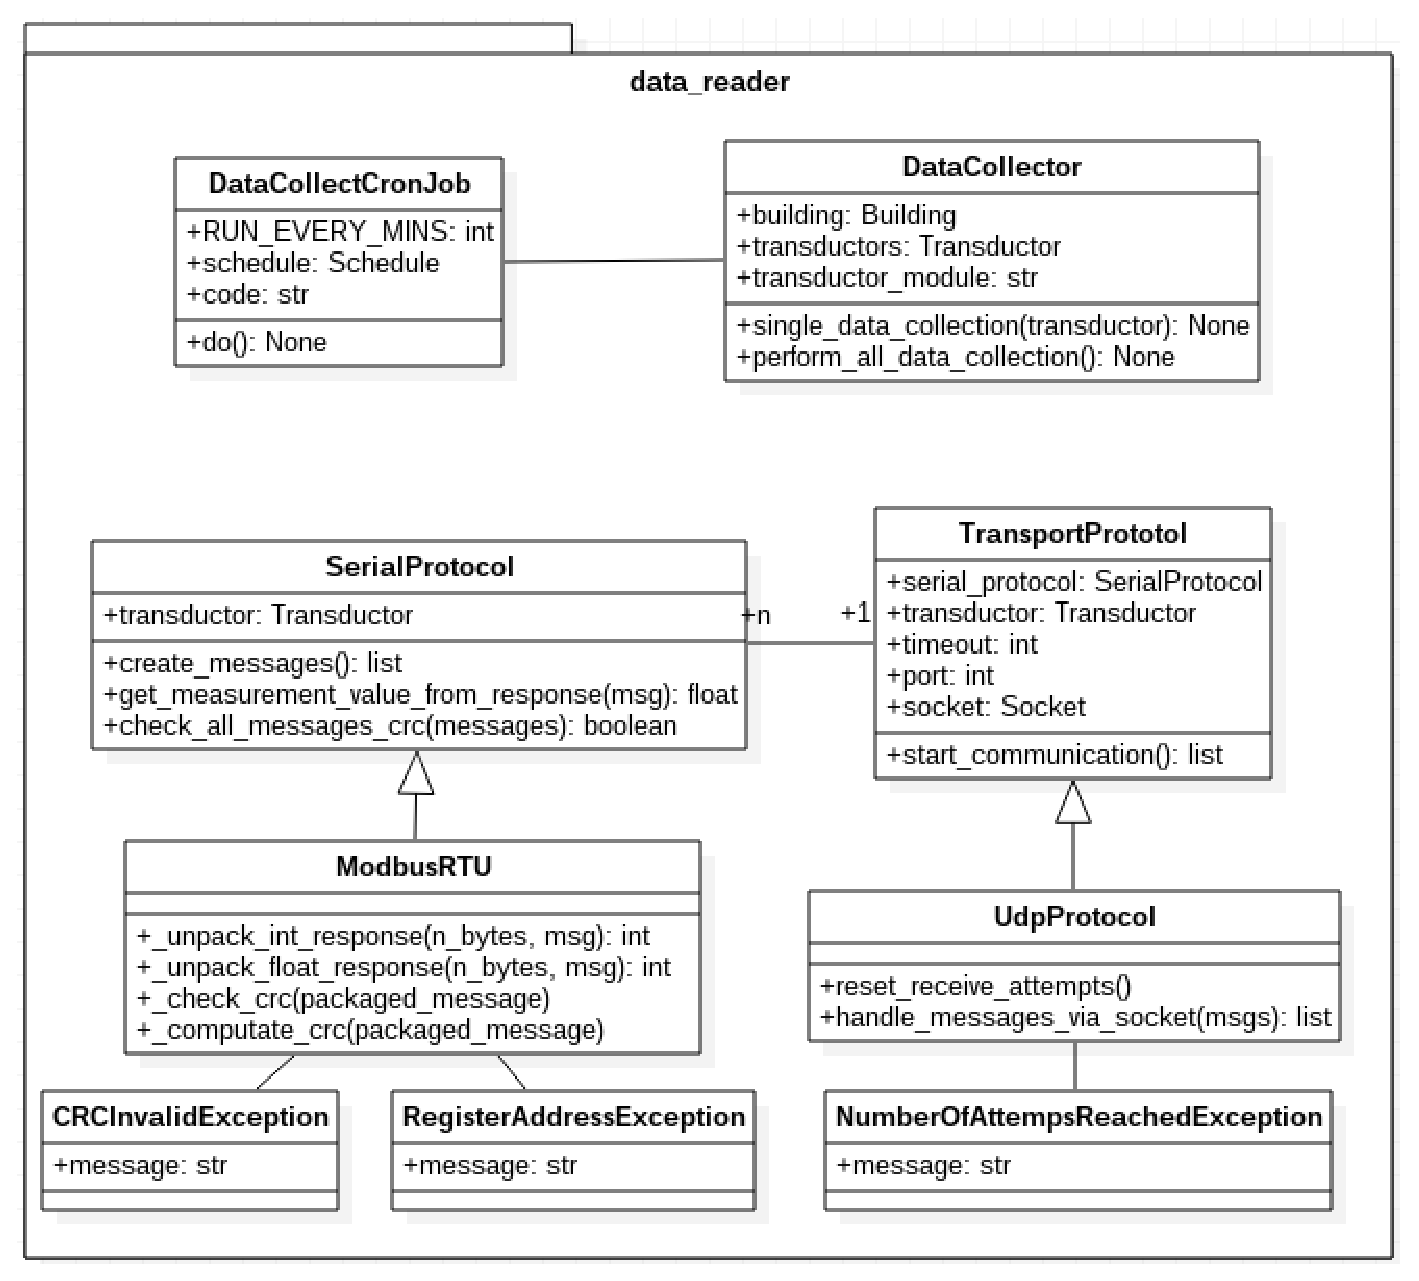
\includegraphics[keepaspectratio=true,scale=0.7]{figuras/data_reader.eps}
    \caption{Diagrama de Classes para \textit{app} \textit{data\_reader}.}
    \label{data_reader}
\end{figure}

A classe \textit{SerialProtocol} e \textit{TransportProtocol} são abstratas e possuem alguns métodos base, para que possa ser possível criar diferentes tipos de especializações, conforme a aplicação necessite. As duas inicialmente criadas, foram referentes aos protocolos Modbus-RTU e UDP.

A coleta de dados para cada prédio, com base no equipamento TR4020, é ilustrada pela Figura \ref{process_1}. Foi utilizada a ferramenta Bizagi\footnote{\url{https://www.bizagi.com/}} para a realização da modelagem.

\begin{figure}[!h]
    \centering
    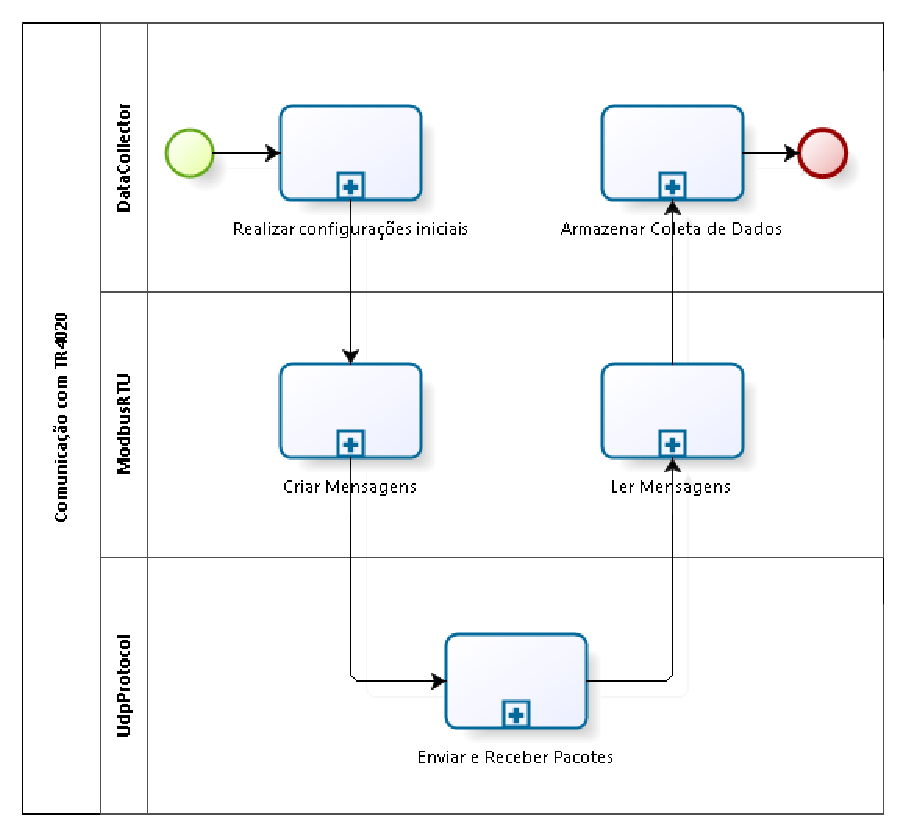
\includegraphics[keepaspectratio=true,scale=1.0]{figuras/process_1.eps}
    \caption{Coleta de dados energéticos utilizando TR4020.}
    \label{process_1}
\end{figure}

Inicialmente, a classe \textit{DataCollector} identifica todos os transdutores que estão no prédio e cria uma \textit{thread} para cada um, objetivando paralelismo na coleta de dados. Segundo Tanembaum \cite{tanenbaum_2007}, as \textit{threads} são entidades escalonadas para a execução sobre a CPU, permitindo que múltiplas execuções ocorram no mesmo ambiente de um processo, com um grande grau de independência uma da outra.

Em cada \textit{thread} é identificado o modelo TR4020 para o transdutor, o qual possui as informações sobre os protocolos Modbus-RTU e UDP. A classe \textit{ModbusRTU} prepara todas as mensagens que deverão ser lidas pelo equipamento, uma para cada grandeza energética e para cada fase. As mensagens seriais criadas são recebidas pela classe \textit{UdpProtocol}, que tentará realizar a comunicação com o aparelho. Os pacotes são enviados e recebidos, um por um, até que todos sejam recebidos corretamente. Com os pacotes recebidos, são extraídas suas cargas úteis, que basicamente correspondem às medições de cada grandeza, logo após, elas são lidas, utilizando a classe \textit{ModbusRTU}. Por fim, a classe \textit{DataCollector} recebe as medições e as salva.

A coleta temporizada, a cada 1 minuto, das medições energéticas realizadas pelos prédios utiliza a ferramenta \verb|cron| \cite{paul_cron}, presente em sistemas UNIX. O \verb|cron| é um \textit{daemon} para executar comandos de agendamento. Um \textit{daemon} é um programa executado em segundo plano e visa estar sempre em execução, caso seja iniciado. Além disso, o \verb|cron| utiliza o \verb|crontab| para manter os arquivos, que possuem instruções a serem executadas periodicamente, de cada usuário. Um arquivo mantido pelo \verb|crontab| deve seguir a estrutura da Figura \ref{crontab_12}.

\begin{figure}[!h]
    \centering
    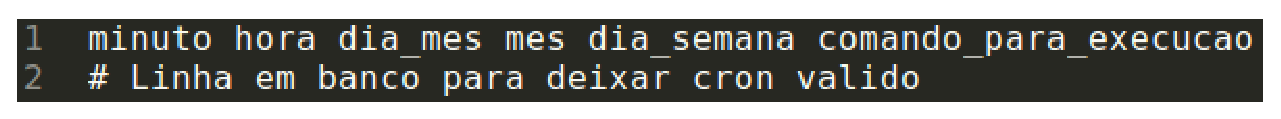
\includegraphics[keepaspectratio=true,scale=0.7]{figuras/crontab.eps}
    \caption{Estrutura de um arquivo mantido pelo \textit{crontab}.}
    \label{crontab_12}
\end{figure}

Adicionou-se um novo comando para a aplicação, chamado \textit{runcrons}. Esse comando é definido pela ferramenta django-cron\footnote{\url{http://django-cron.readthedocs.io/en/latest/}} e basicamente executa um código que possua como base a classe \textit{CronJobBase}. Esse código, após ser executado, é bloqueado até que o tempo de espera para outra execução seja atingido, como uma espécie de cronômetro.

Criou-se a classe \textit{DataCollectCronJob}, Algoritmo \ref{data_collect}, objetivando invocar o \textit{DataCollector} para realizar a coleta de dados. O arquivo mantido pelo crontab para realizar a coleta, periodicamente a cada 1 minuto, foi definido conforme o Algoritmo \ref{cron_slave}.

\begin{python}[caption={Classe \textit{DataCollectCronJob}.}, captionpos=b, label={data_collect}]
class DataCollectCronJob(CronJobBase):
    RUN_EVERY_MINS = 0
    schedule = Schedule(run_every_mins=RUN_EVERY_MINS)
    code = 'smi_unb.data_reader.cronjob.DataCollectCronJob'

    def do(self):
        data_collector = DataCollector()
        data_collector.perform_all_data_collection()
\end{python}

\begin{python}[caption={\textit{Cron} para execução da coleta dos dados de energia.}, captionpos=b, label={cron_slave}]
* * * * * python3 /SMI-UnB/manage.py runcrons \
smi_unb.data_reader.cronjob.DataCollectCronJob
# Necessary line at end of file to make cron valid
\end{python}

\subsection{Servidor Mestre}
O servidor mestre é responsável por realizar uma sincronização de entidades e medições de energias utilizando uma API \textit{web}. Ressalta-se que a sincronização de entidades será explicada na próxima sessão.

\textit{Application Programming Interface} (API) é um conjunto de requisitos que regem como um aplicativo pode conversar com outro. As APIs realizam isso expondo algumas das funções internas de um programa para o mundo exterior de forma limitada, possibilitando que os aplicativos compartilhem dados e tomem ações em nome do outro, sem exigir que os desenvolvedores compartilhem todo o código do \textit{software} \cite{brian_api}.

Quando usado no contexto do desenvolvimento \textit{web}, uma API é tipicamente definida como um conjunto de requisições do protocolo HTTP, juntamente com uma definição da estrutura de mensagens de resposta, geralmente utilizando as linguagens \textit{Extensible Markup Language} (XML) ou \textit{JavaScript Object Notation} (JSON) \cite{benslimane_2008}.

O \textit{Hypertext Transfer Protocol} (HTTP), é um protocolo \textit{web} presente na camada de aplicação do modelo OSI e é implementado por dois programas: um cliente e outro servidor. Os programas cliente e servidor conversam entre si, trocando mensagens HTTP, sendo que o protocolo define como o cliente (por exemplo, um navegador) solicitará páginas \textit{web} de um servidor (por exemplo, o Django) e como o servidor irá transferir essas páginas para o cliente \cite{kurose_2002}.

A API utilizada no projeto baseou-se no Django REST Framework \cite{django_rest}. O \textit{Representational State Transfer} (REST) \cite{fielding_2000} é um estilo arquitetural para projetar sistemas distribuídos e apresenta as seguintes características:

\begin{itemize}
    \item Estado e funcionalidade são divididos em recursos distribuídos;
    \item Todo recurso é exclusivamente endereçável, usando um conjunto uniforme e mínimo de comandos;
    \item O protocolo é cliente/servidor, sem estado, em camadas e suporta armazenamento em \textit{cache}.
\end{itemize}

O Django REST Framework utiliza alguns métodos HTTP para mapear as operações CRUD (criar, resgatar, atualizar e deletar) nas requisições HTTP, sendo estes:

\begin{itemize}
    \item GET: recuperar informações de uma entidade;
    \item POST: criar ou atualizar uma entidade;
    \item PUT: criar ou atualizar uma entidade. O método PUT é idempotente, ou seja, se uma operação for realizada duas vezes sobre o mesmo objetivo, não haverá efeito;
    \item PATCH: modificar parcialmente uma entidade;
    \item DELETE: deletar uma entidade.
\end{itemize}

O conceito de \textit{endpoints} é utilizado pelo Django REST Framework, objetivando a interação com a API do lado do servidor, pois especificam onde os recursos podem ser acessados. Uma das classes padrão utilizada no projeto foi a \textit{ModelViewSet}. Além disso, o Django REST Framework utiliza serializadores. Os serializadores permitem que dados complexos, como \textit{querysets} e instâncias de modelos, sejam convertidos em tipos de dados Python nativos que podem ser facilmente processados em JSON, XML ou outros tipos de conteúdo. Os serializadores também fornecem desserialização, permitindo que os dados analisados sejam convertidos novamente em tipos complexos, após realizada uma validação dos dados recebidos \cite{django_rest}.

Realiza-se a sincronia de dados por meio da classe \textit{EnergyMeasurementSynchronizer}, presente no \textit{app} \textit{api}, Figura \ref{api}. Em linhas gerais, essa classe realiza duas requisições HTTP para cada servidor escravo. Na primeira requisição são consumidas as medições de energia mais recentes de cada transdutor, via API. Com as medições resgatadas, atualiza-se o horário da última coleta de dados de cada transdutor, no servidor mestre. Após atualizados os horários no mestre, realiza-se a segunda requisição, que atualiza o horário da última coleta de dados de todos os transdutores presentes no escravo.

\begin{figure}[!h]
    \centering
    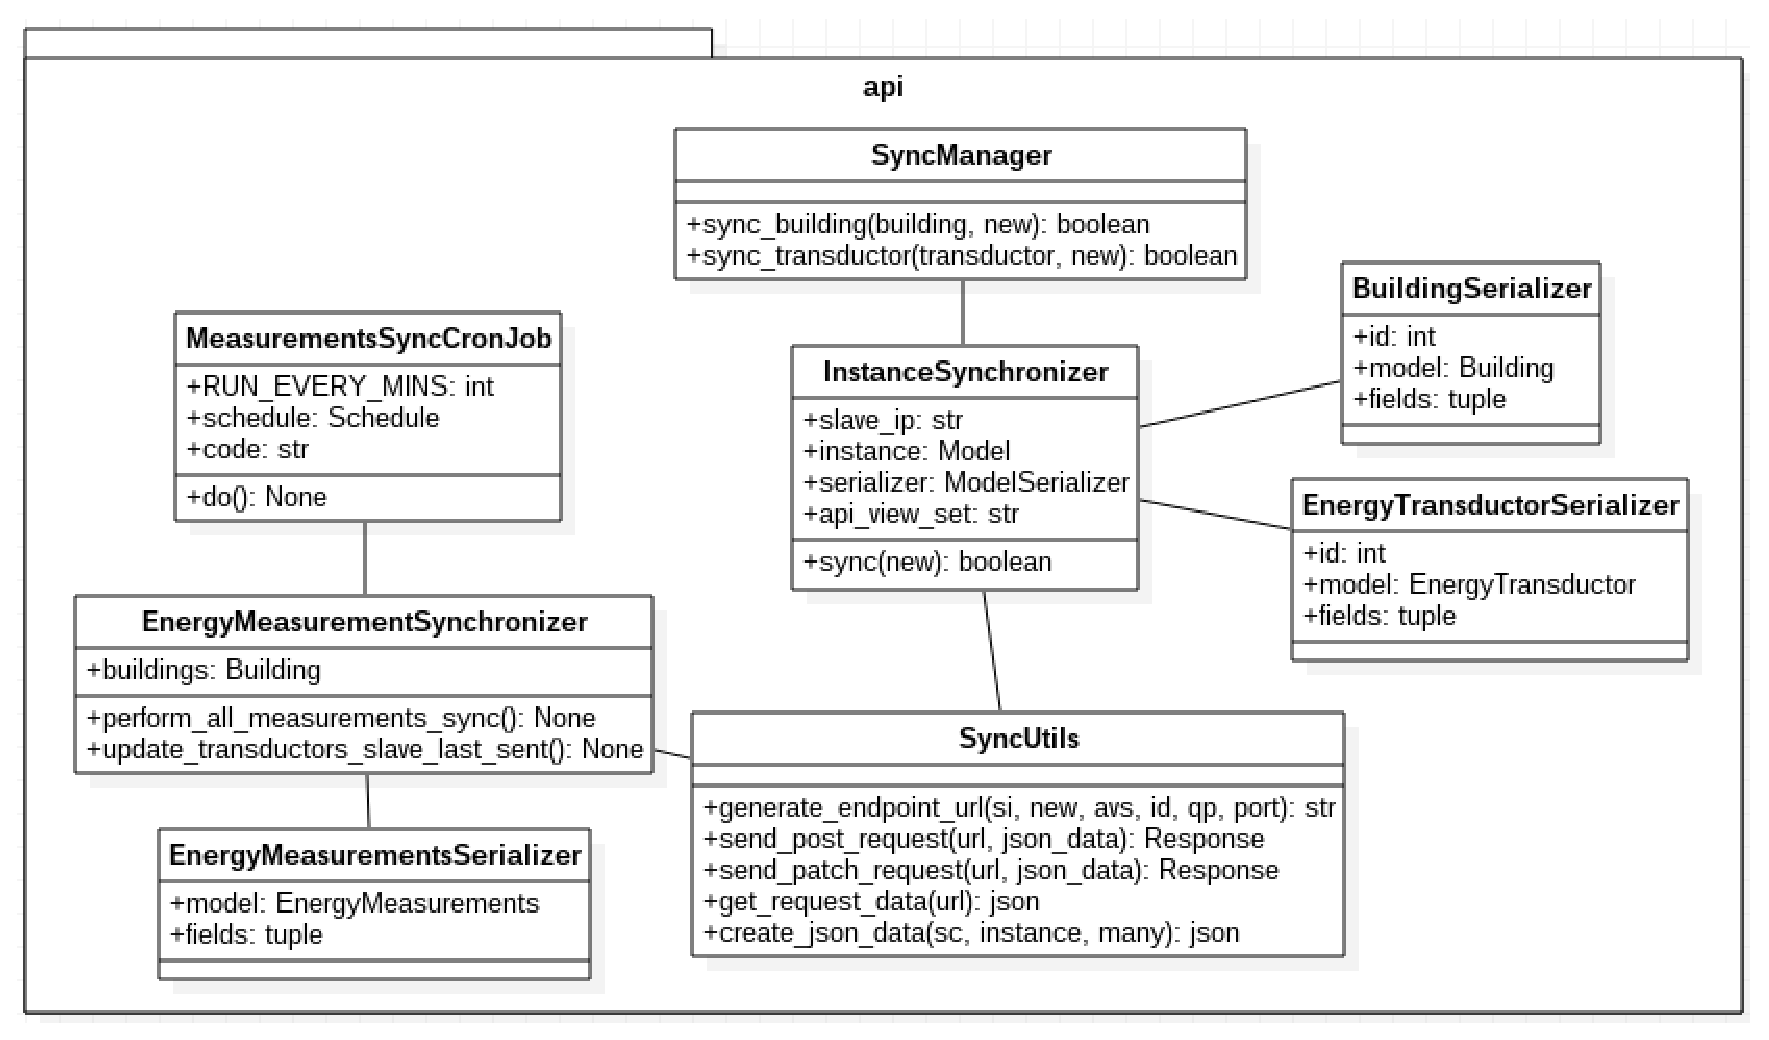
\includegraphics[keepaspectratio=true,scale=0.55]{figuras/api.eps}
    \caption{Diagrama de Classes para \textit{app} \textit{api}.}
    \label{api}
\end{figure}

O \verb|crontab| para se realizar a sincronia das medições, a cada 1 hora, é expresso pelo Algoritmo \ref{cron_master} e utiliza a classe \textit{MeasurementsSyncCronJob}, Algoritmo \ref{measu_sync}.

A base da API foi realizada com sucesso, para que no futuro haja apenas aprimoramentos, como a sua autenticação e hiperlincamento, conforme recomendado pelo Django REST Framework.

\begin{python}[caption={\textit{Cron} para execução da sincronia dos dados de energia.}, captionpos=b, label={cron_master}]
0 * * * * python3 /SMI-UnB/manage.py runcrons \
smi_unb.api.cronjob.MeasurementsSyncCronJob
# Necessary line at end of file to make cron valid
\end{python}

\begin{python}[caption={Classe MeasurementsSyncCronJob.}, captionpos=b, label={measu_sync}]
class MeasurementsSyncCronJob(CronJobBase):
    RUN_EVERY_MINS = 59
    schedule = Schedule(run_every_mins=RUN_EVERY_MINS)
    code = 'smi_unb.api.cronjob.MeasurementsSyncCronJob'

    def do(self):
        e_synchronizer = EnergyMeasurementSynchronizer()
        e_synchronizer.perform_all_measurements_sync()
\end{python}

\section{Segurança em Geral}
Realizou-se um sistema de \textit{login} por meio de e-mail, para facilitar os usuários a se autenticarem no sistema. O Django já possui um módulo de autenticação bem definido, que realiza tanto a autenticação quanto a autorização de um usuário. Como esse módulo realizava \textit{login} por meio do nome de usuário, algumas mudanças foram implementadas para ser possível o \textit{login} por meio de e-mail. Para isso, criou-se o \textit{app} \textit{authentication}, Figura \ref{authentication}, o qual define a classe \textit{EmailBackend}, que por sua vez realiza a autenticação por e-mail.

\begin{figure}[!h]
    \centering
    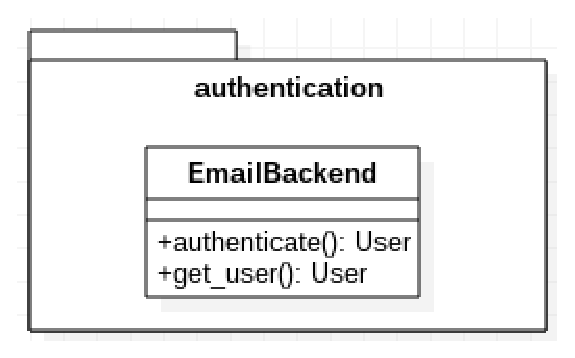
\includegraphics[keepaspectratio=true,scale=0.8]{figuras/authentication.eps}
    \caption{\textit{App} authentication}
    \label{authentication}
\end{figure}

Os transdutores e prédios presentes no sistema não podem ser excluídos, tendo em vista a importância de se deixar registrado suas medições realizadas. Para isso acontecer, alguns botões de habilitar e desabilitar foram adicionados à aplicação e um atributo referente a ativo foi adicionado aos seus modelos.

O servidor mestre é responsável por realizar todo o registro, edição, ativação e desativação de transdutores e prédios. Assim, sempre que se tenta realizar uma operação desse tipo, o mestre realiza uma verificação, a nível de formulário, com o escravo. Essa verificação é feita por meio de uma requisição HTTP, utilizando o método GET e possui um \textit{timeout} configurável. Caso o código de resposta recebido seja válido, o mestre tenta realizar uma sincronização com escravo via API, utilizando a classe \textit{SyncManager}, Figura \ref{api}. Ressalta-se que esta solução é um protótipo e deve ser aperfeiçoada, buscando aceitar requisições mais seguras, por meio do protocolo HTTPS.

Definiu-se, inicialmente, duas permissões para os usuários: gerência de prédios e de transdutores. Cada uma dessas fornece ao usuário os direitos de incluir, modificar e habilitar/desabilitar. A gerência de usuários e definição das permissões são realizadas pelo \textit{app} \textit{users}, Figura \ref{app_users}.

\begin{figure}[!h]
    \centering
    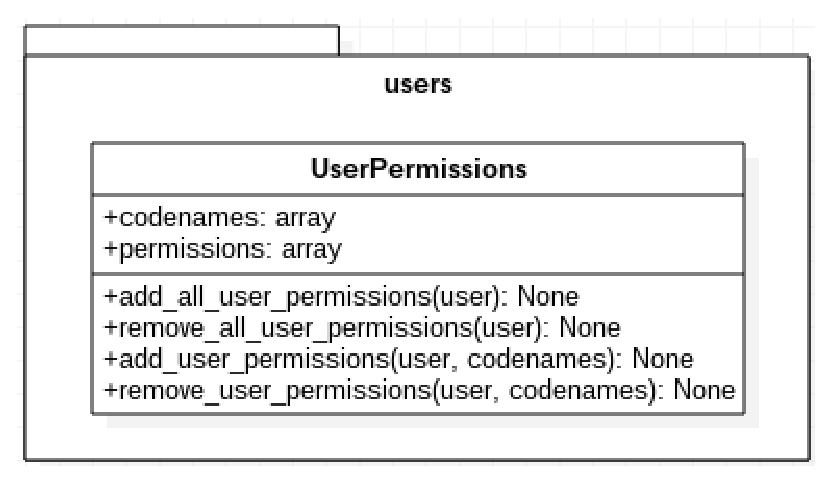
\includegraphics[keepaspectratio=true,scale=0.8]{figuras/app_users.eps}
    \caption{Diagrama de Classes para \textit{App} \textit{users}.}
    \label{app_users}
\end{figure}

\section{Gerência de Configuração}

\subsection{Docker}
Criaram-se duas configurações para os ambientes referentes ao mestre e escravo, onde suas diferenciações baseavam-se no \verb|crontab| que seria executado em cada um. Para realizar essas configurações, utilizou-se a ferramenta Docker Compose, tornando mais fácil a definição e execução de múltiplos contêiners, com uma possibilidade de ligação entre eles. Os serviços definidos para a aplicação foram:

\begin{itemize}
    \item nginx: fornecimento dos arquivos estáticos;
    \item web: fornecimento da aplicação em Django;
    \item postgres: armazenamento das informações;
    \item redis: \textit{cache} da aplicação;
    \item data: armazenamento do banco de dados.
\end{itemize}

A configuração para o servidor mestre é representada pelo Algoritmo \ref{compose_docker}.

\begin{python}[caption={Serviços providos pelo Docker Compose.}, captionpos=b, label={compose_docker}]
version: '2'
services:
  nginx:
    restart: always
    build: ./docker/nginx/
    ports:
      - "80:80"
    volumes:
      - ./docker/nginx/collect/static/:/var/www/static/
    volumes_from:
      - web
    links:
      - web:web

  web:
    build:
      context: .
      dockerfile: ./docker/Dockerfile.master
    expose:
      - "8000"
    links:
      - postgres:postgres
      - redis:redis
    env_file: ./docker/env
    volumes:
      - ./src/:/app/src/

  postgres:
    restart: always
    image: postgres:latest
    volumes_from:
      - data
    volumes:
      - ./docker/postgres/docker-entrypoint-initdb.d: \
         /docker-entrypoint-initdb.d
    env_file:
      - ./docker/env
    expose:
      - "5432"

  redis:
    restart: always
    image: redis:latest
    expose:
      - "6379"

  data:
    restart: always
    image: alpine
    volumes:
      - /var/lib/postgresql
    command: "true"
\end{python}

O serviço nginx utiliza um servidor nginx\footnote{\url{https://nginx.org/en}} para lidar primeiramente com requisições externas e fornecer os arquivos estáticos da aplicação. O nginx consiste em um servidor HTTP e \textit{proxy} reverso. Servidores \textit{proxy} reverso utilizam um servidor \textit{proxy} para atuar como um intermediadores entre uma requisição realizada por um cliente e o servidor que a atenderá. Um servidor \textit{proxy} é uma entidade de rede que satisfaz solicitações HTTP em nome de um cliente, possuindo seu próprio armazenamento em disco e mantendo cópias de objetos recentemente solicitados \cite{kurose_2002}.

Requisições que precisam ser geradas dinamicamente são tratadas pelo serviço \textit{web}, que são enviadas para um servidor Gunicorn\footnote{\url{http://gunicorn.org/}}. O Gunicorn é um servidor Python \textit{Web Server Gateway Interface} (WSGI) HTTP. O WSGI é uma especificação para uma interface simples e universal entre servidores \textit{web} e aplicações \textit{web} ou \textit{frameworks} para a linguagem de programação Python \cite{pep_333}.

Quando o serviço \textit{web} é iniciado, executa-se um \textit{script}, Algoritmo \ref{script_start}, responsável por criar um arquivo contendo as variáveis de ambiente, popular o banco de dados com os \textit{campi} da UnB e os modelos de transdutor base, inicializar o \textit{daemon} \verb|cron| e o servidor Gunicorn.

\begin{python}[caption={\textit{Script} \textit{start.sh}.}, captionpos=b, label={script_start}]
#!/bin/bash

# Creating file with environment variables to use in crontab
env | sed 's/^\(.*\)$/ \1/g' > /root/env

# Populating database and initializing cron and gunicorn
python3 manage.py makemigrations && \
python3 manage.py migrate && \
python3 manage.py loaddata src/smi_unb/fixtures/initial_data.json && \
cron && \
gunicorn smi_unb.wsgi -b 0.0.0.0:8000
\end{python}

A criação do arquivo contendo as variáveis de ambiente é necessária, pois o \verb|crontab| de um contêiner não possui acesso a elas. Os \textit{crontabs} dos servidores mestres e escravo realizam uma exportação das variáveis antes de executarem seus devidos comandos. O Algoritmo \ref{crontab_master} ilustra o \verb|crontab| do servidor mestre.

\begin{python}[caption={\textit{Crontab} do servidor mestre.}, captionpos=b, label={crontab_master}]
0 * * * * export $(cat /root/env | xargs) && \
python3 /app/manage.py runcrons \
smi_unb.api.cronjob.MeasurementsSyncCronJob
# Necessary line at end of file to make cron valid
\end{python}

O serviço \textit{postgres} utiliza uma imagem banco de dados PostgreSQL para realizar o armazenamento das informações.

Para acelerar as requisições de páginas \textit{web} do SMI-UnB, utilizou-se o serviço \textit{redis}, responsável por executar um servidor Redis\footnote{\url{https://redis.io/}}. O \textit{Cache} é um componente de \textit{hardware} ou \textit{software} que armazena dados, objetivando uma maior rapidez para pedidos futuros. Os dados armazenados em um \textit{cache} podem ser o resultado de uma computação executada anteriormente ou da duplicação de dados presentes em um outro lugar \cite{hennessy_2011}.

O serviço \textit{data} foi utilizado para gerenciar a persistência de dados, objetivando não arriscar qualquer exclusão acidental durante, por exemplo, uma atualização no contêiner do PostgreSQL.

Criou-se um \textit{script}, Algoritmo \ref{script_postgres}, responsável por criar um arquivo contendo as variáveis de ambiente referentes ao banco de dados.

\begin{python}[caption={\textit{Script} \textit{db\_initial\_data.sh}.}, captionpos=b, label={script_postgres}]
#!/bin/bash
echo "Collecting data to create the database..."

read -p "Enter the database name: " db_name

read -p "Enter the database user: " db_user

while true; do
    read -s -p "Enter the database password: " db_pass
    echo
    read -s -p "Confirm the database password: " db_pass_confirm
    [ "$db_pass" = "$db_pass_confirm" ] && break
    echo -e "\nPasswords don't match. Please try again...\n"
done

file="./docker/env"

if [ -f "$file" ]
then
    rm "$file"
fi

printf "DB_NAME=$db_name\nDB_USER=$db_user\nDB_PASS=$db_pass
        \nDB_SERVICE=postgres\nDB_PORT=5432" >> "$file"

echo -e "\nDatabase configuration created succefully!"
\end{python}

Algumas \textit{tasks} foram adicionadas ao projeto, com auxílio da ferramenta Invoke\footnote{\url{http://www.pyinvoke.org/}}, para facilitarem na execução de comandos longos e serviços do SMI-UnB. Por exemplo, para criar um ambiente de produção do servidor mestre seria necessário seguir os seguintes passos:

\begin{itemize}
    \item Executar \textit{script} para variáveis de ambiente do banco de dados;
    \item Montar os contêiners do SMI-UnB;
    \item Iniciar os contêiners.
\end{itemize}

Em vez de executar os comandos individualmente, esses são agrupados em uma \textit{task} chamada \textit{install\_master}, Algoritmo \ref{task_install_master}, responsável por executá-los sequêncialmente.

\begin{python}[caption={\textit{Task} \textit{install\_master}, presente no arquivo \textit{tasks.py}.}, captionpos=b, label={task_install_master}]
@task
def install_master(ctx):
    print('Installing Master Docker')

    # Database configuration
    subprocess.call(['./scripts/db_initial_data.sh'])

    # Building docker containers
    run('docker-compose -f docker-compose-master.yml build
         --force-rm')

    # Initializing containers
    run('docker-compose -f docker-compose-master.yml up -d')
\end{python}

Além da \textit{task} explicada anteriormente, outras \textit{tasks} referentes à inicialização/encerramento do Docker Compose e do ambiente de desenvolvimento também foram realizadas.

\subsection{Integração Contínua}
O script de integração contínua do projeto, Algoritmo \ref{integracao}, utiliza imagens oficiais do Python 3.5 e do PostgreSQL, presentes no Docker-Hub\footnote{\url{https://hub.docker.com/}}, que é repositório oficial de imagens do Docker. Todas as imagens do docker-hub já estão prontas para serem executadas em contêiners. Após os contêiners serem iniciados e vinculados, é realizada a instalação dos pacotes utilizados pelo SMI-UnB. Com a instalação dos pacotes, inicia-se verificação das normas da PEP8, com a ferramenta flake8 e por fim, são executados todos os testes do sistema e exibida a cobertura total, por meio da ferramenta Coverage\footnote{\url{https://pypi.python.org/pypi/coverage/}}. A \textit{build} da integração contínua irá falhar caso ocorra qualquer erro nos procedimentos informados.

\begin{python}[caption={\textit{Script} para integração contínua do projeto.}, captionpos=b, label={integracao}]
image: "python:3.5"

services:
  - postgres:latest

variables:
  POSTGRES_DB: smiunbtest
  POSTGRES_USER: postgres
  POSTGRES_PASSWORD: ""

test:
    script:
        - apt-get update -qq
        - apt-get install python3-pip -y -qq
        - pip3 install -e .[dev]
        - flake8 src/ --exclude migrations
        - coverage run manage.py test smi_unb \
          --settings=smi_unb.settings_runner
        - coverage report
\end{python}

\section{Apresentação das Informações}
O \textit{framework} Bootstrap foi utilizado como base para se realizar o \textit{layout} da aplicação, por possuir estruturas bem definidas e fáceis de serem utilizadas. Utilizou-se o jQuery\footnote{\url{https://jquery.com/}} para facilitar o uso de \textit{javascripts} na aplicação. Os ícones presentes foram provenientes do Font Awesome\footnote{\url{http://fontawesome.io/}}. As três bibliotecas são disponilizados sobre uma licença livre e podem ser utilizados em qualquer projeto, contanto que haja uma referência sobre elas.

Ressalta-se que não foi realizado nenhum teste de usabilidade para a aplicação. Os princípios de usabilidade utilizados partiram de conhecimentos do próprio autor, adquiridos através de conceitos da literatura e experiências pessoais.

A página inicial do SMI-UnB, Figura \ref{main_page}, utiliza uma imagem gratuita do site \textit{FreeImages}\footnote{\url{http://pt.freeimages.com}}, disponibilizada sob sua licença\footnote{\url{http://pt.freeimages.com/license}}. O \textit{site} e o criador, Friedrich Plechschmidt, possuem todos os direitos de propriedade intelectual sobre a imagem.

\begin{figure}[!h]
    \centering
    
\includegraphics[scale=0.35]{figuras/main_page.eps}
    \caption{Página inicial do SMI-UnB.}
    \label{main_page}
\end{figure}

Foram definidas duas páginas principais para o SMI-UnB: painel de controle e ``minha conta''. O painel de controle, Figura \ref{dashboard}, possui como intuito unir os principais recursos do sistema de uma maneira fácil e rápida, para que o usuário não perca muito tempo até encontrá-los. A página ``minha conta'', Figura \ref{my_account}, possui as opções para o gerenciamento das informações de um usuário específico, como a alteração das informações básicas e mudança de senha.

\begin{figure}[!h]
    \centering
    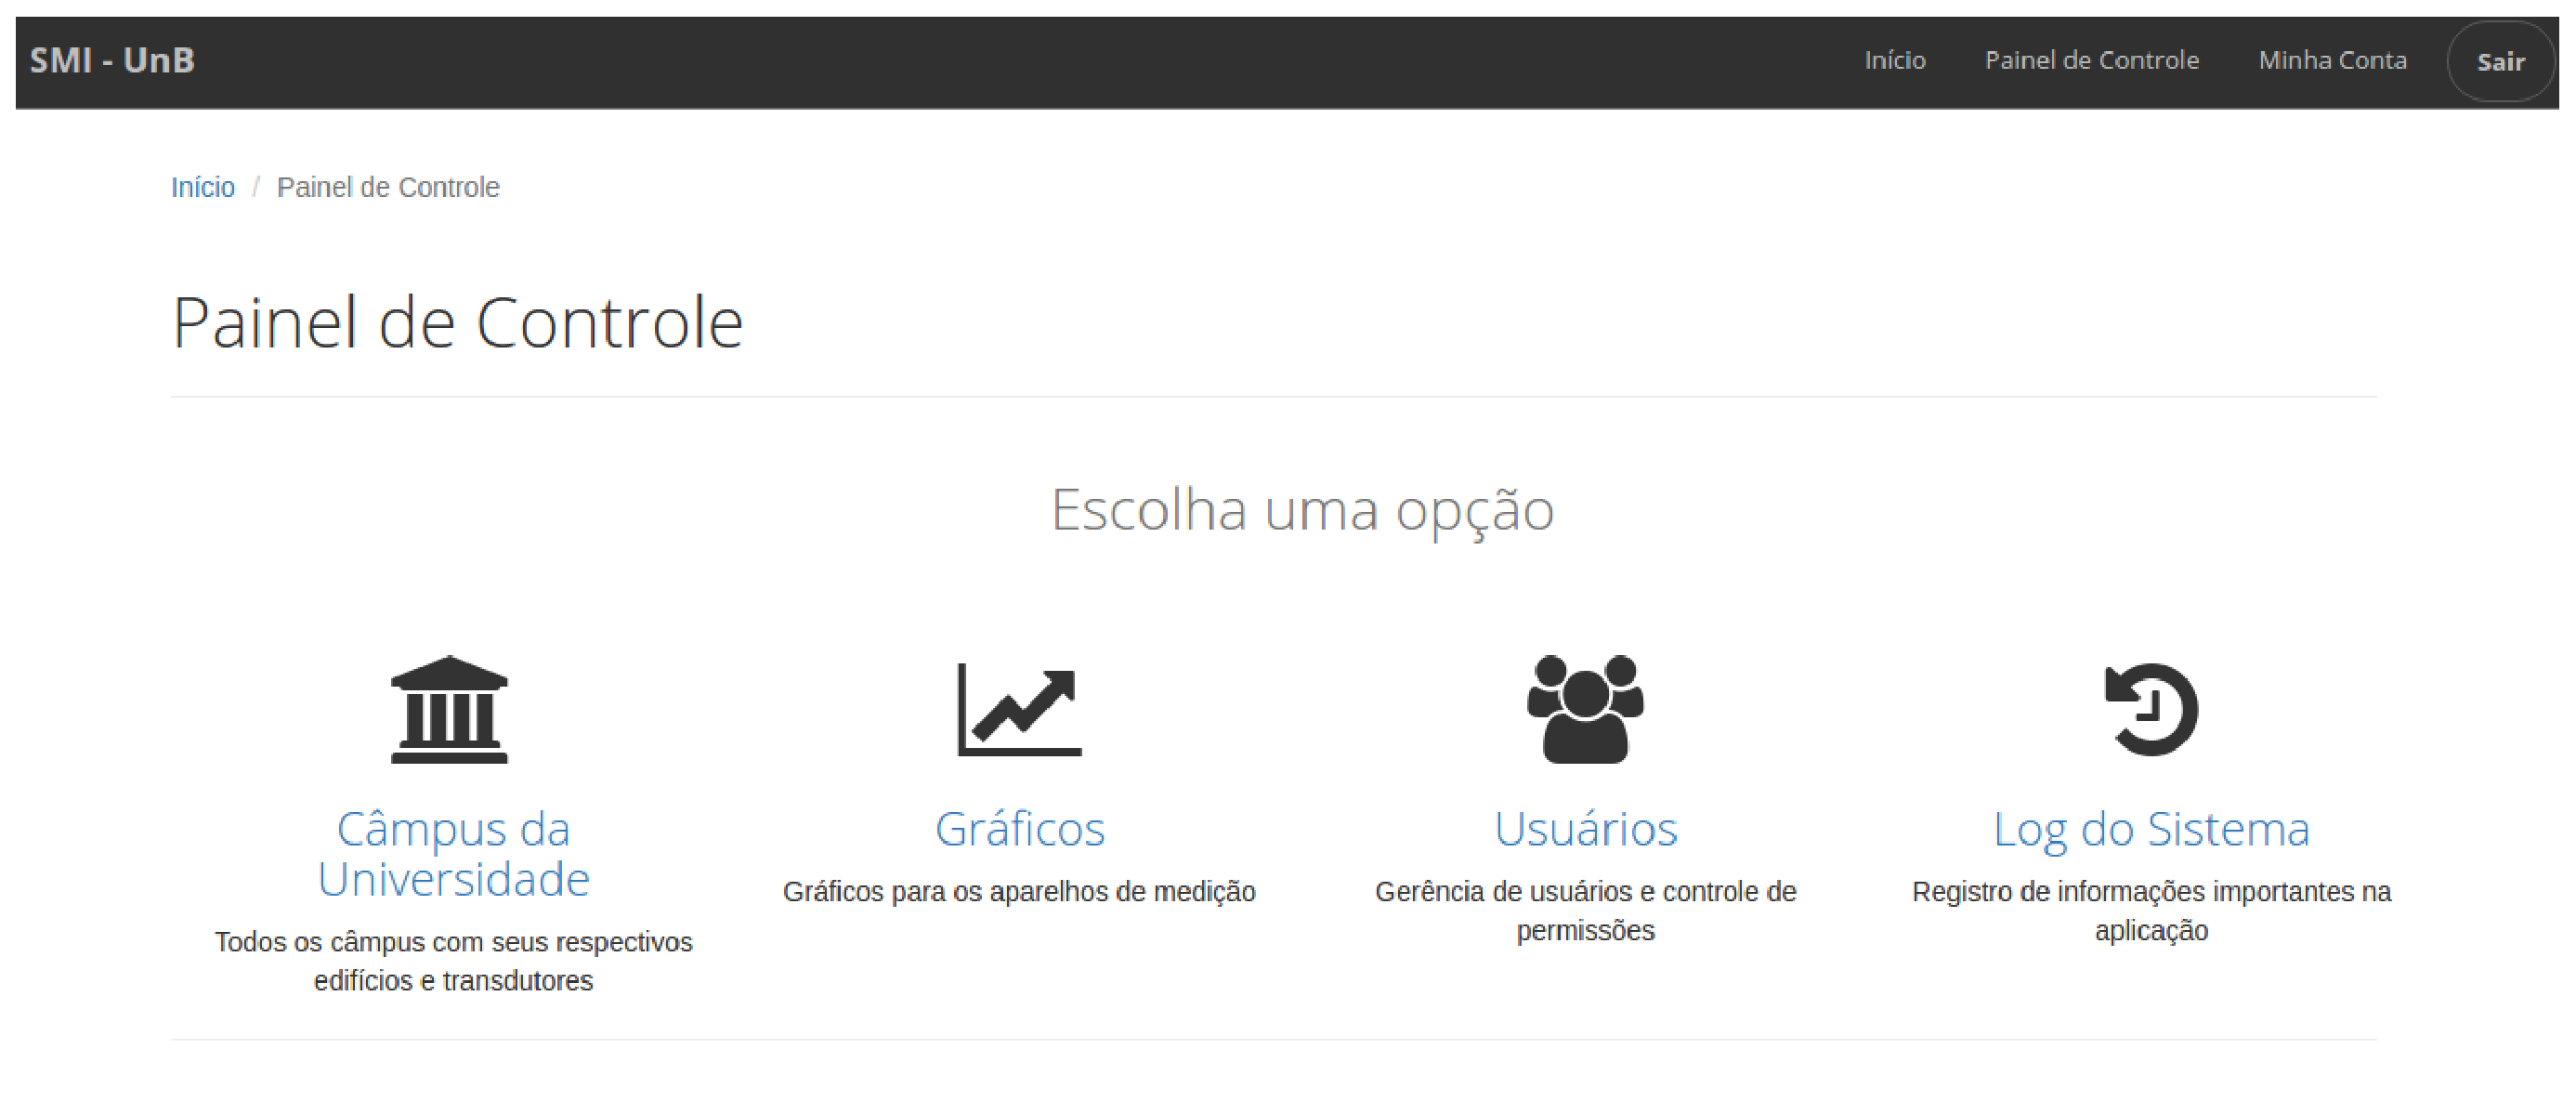
\includegraphics[scale=0.35]{figuras/dashboard.eps}
    \caption{Página do painel de controle do SMI-UnB.}
    \label{dashboard}
\end{figure}

\begin{figure}[!h]
    \centering
    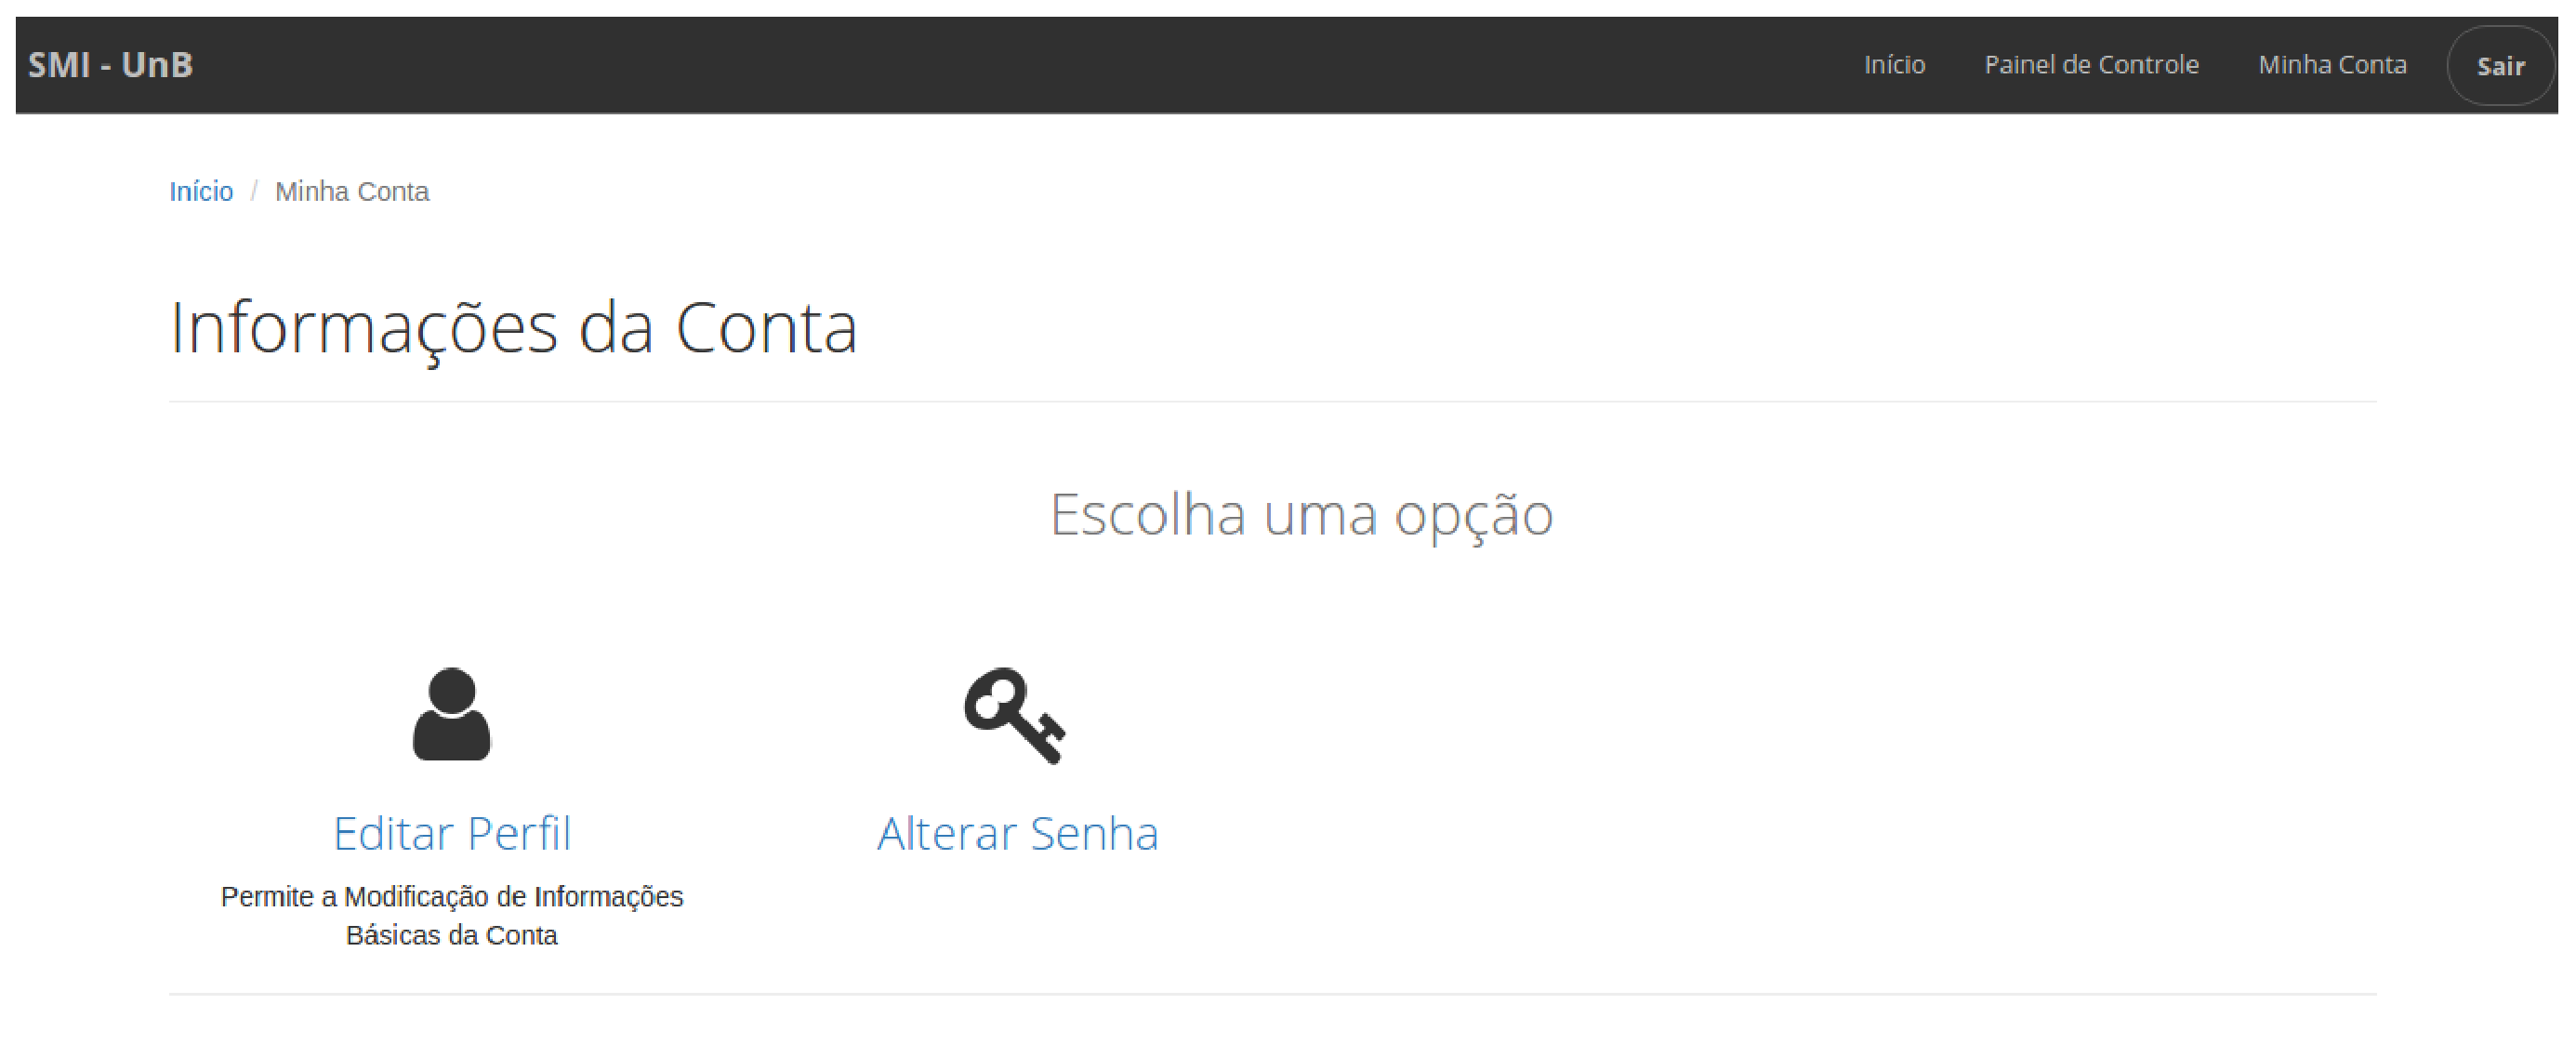
\includegraphics[scale=0.35]{figuras/my_account.eps}
    \caption{Página para gerenciamento de informações de um usuário.}
    \label{my_account}
\end{figure}

Os botões da aplicação, Figuras \ref{buttons} e \ref{buttons_2}, possuem cores e nomes bem significativos, auxiliando o usuário a realizar uma operação com maior segurança. Por exemplo, a cor verde para um botão indica que um registro/ativação será realizado, a cor amarela indica uma alteração e a vermelha uma desativação. Além disso, as operações de criar, atualizar, habilitar ou desabilitar necessitam de uma confirmação provinda do usuário, objetivando essas não sejam realizadas de maneira indevida.

\begin{figure}[!h]
    \centering
    
\includegraphics[scale=0.4]{figuras/buttons.eps}
    \caption{Botões presentes na página de um campus.}
    \label{buttons}
\end{figure}

\begin{figure}[!h]
    \centering
    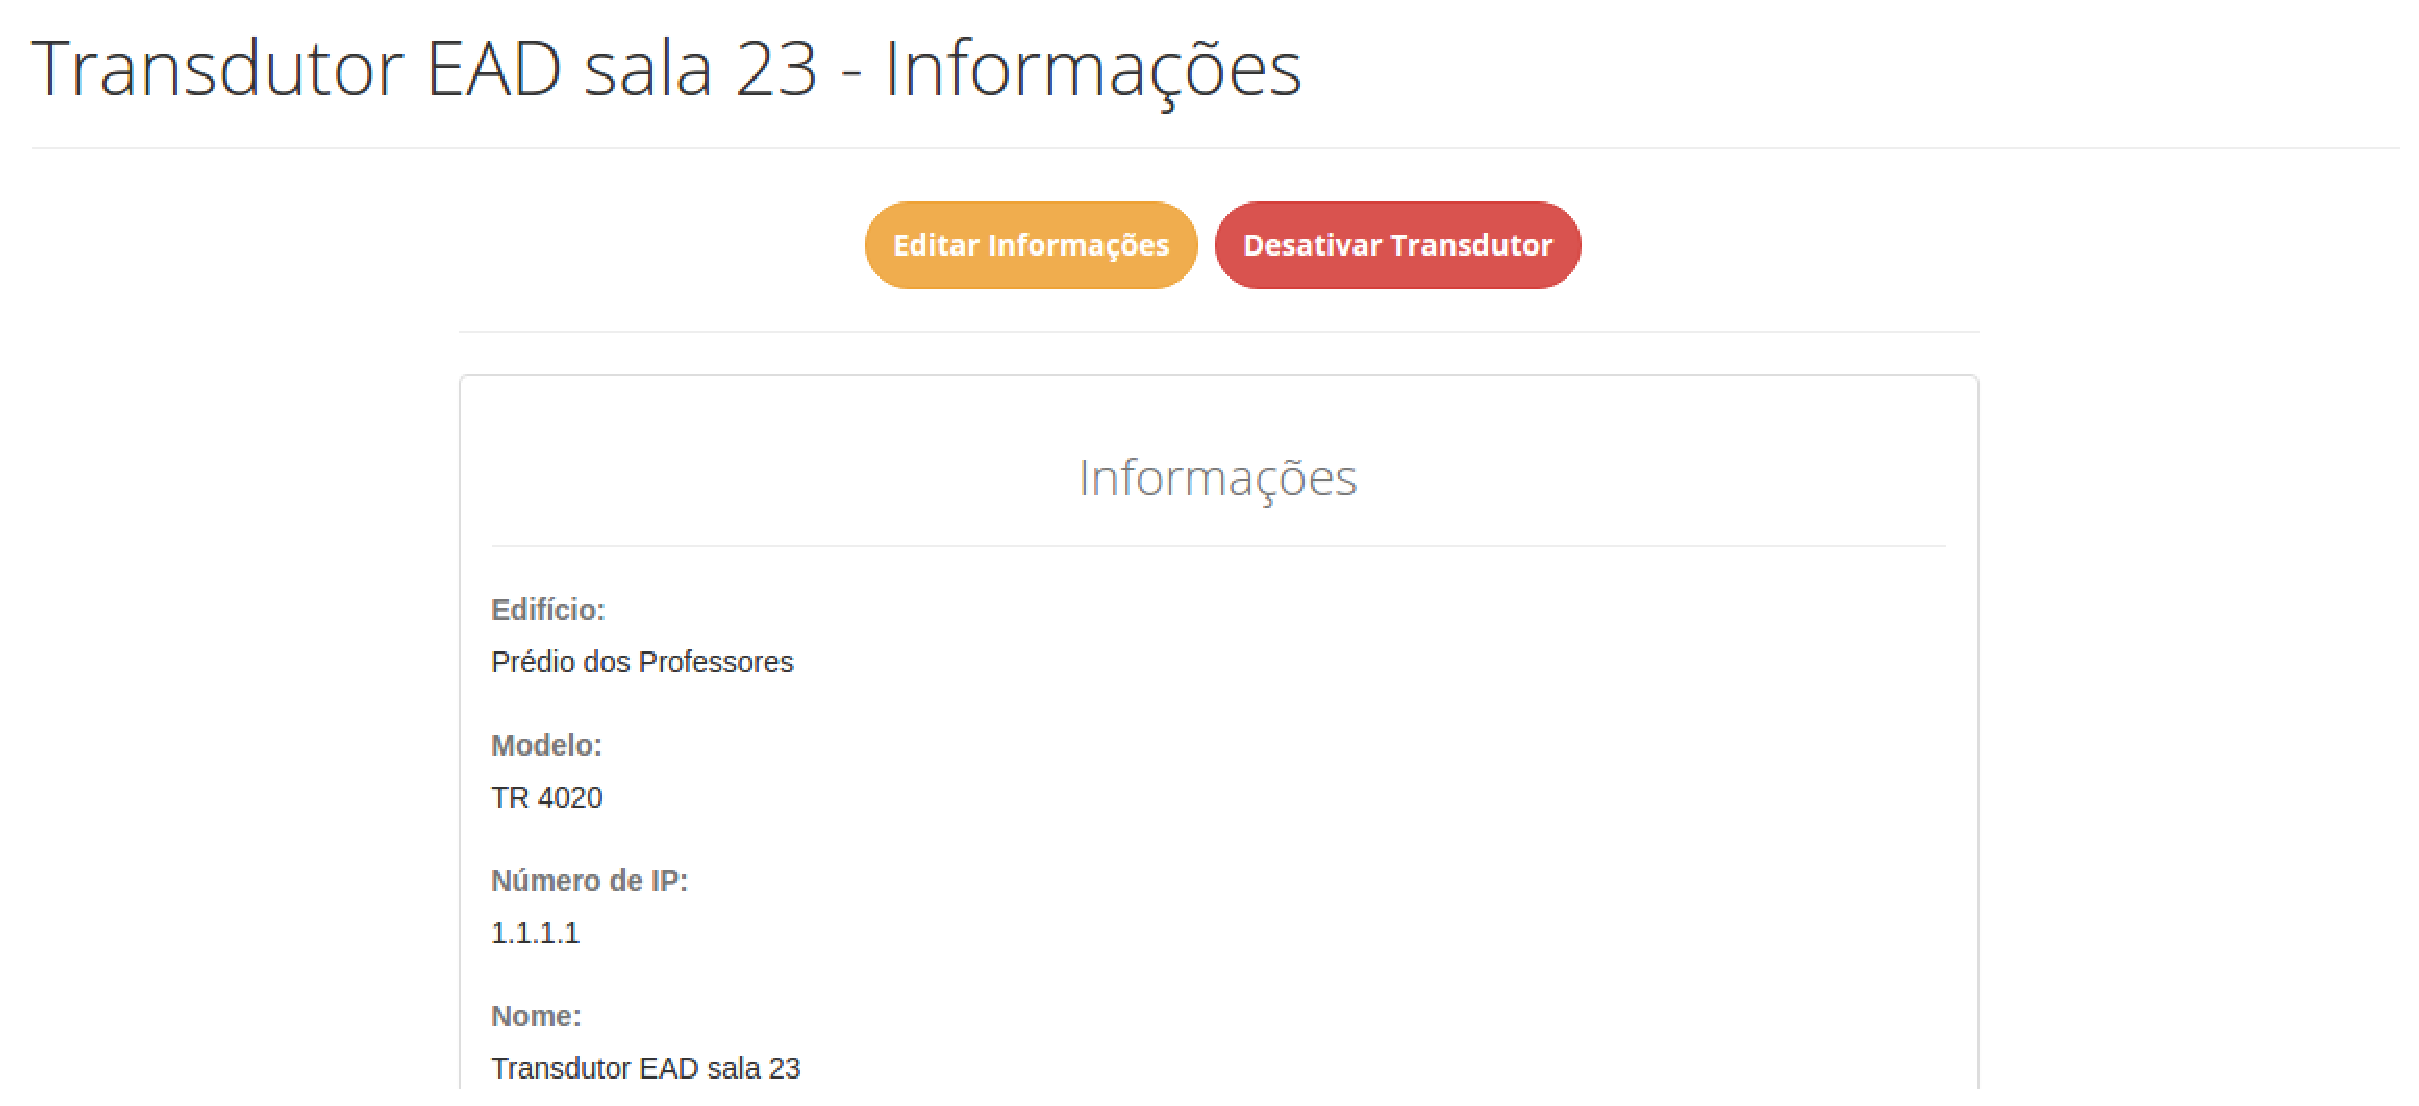
\includegraphics[scale=0.4]{figuras/buttons_2.eps}
    \caption{Botões presentes na página de um transdutor.}
    \label{buttons_2}
\end{figure}

As páginas do sistema possuem \textit{breadcrumbs}\footnote{Elemento de controle gráfico usado como ajuda de navegação em interfaces de usuário.}, Figura \ref{links}, que mapeiam onde o usuário se encontra e quais são as páginas anteriores a essa. Assim, dificilmente o usuário irá se perder na aplicação.

\begin{figure}[!h]
    \centering
    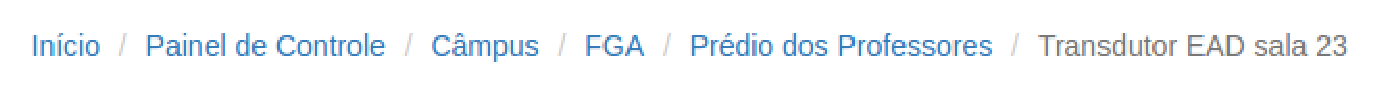
\includegraphics[scale=0.7]{figuras/links.eps}
    \caption{\textit{Breadcrumbs} para página de um transdutor específico.}
    \label{links}
\end{figure}

As demais imagens do SMI-UnB encontram-se no apêndice.

\subsection{Gráfico de Linhas}
Realizou-se um gráfico de linhas com auxílio do app \textit{report}, Figura \ref{app_report}, para que fosse possível apresentar as informações energéticas ao usuário de maneira prática e intuitiva. A biblioteca utilizada para criar o gráfico foi a \textit{matplotlib}\footnote{\url{https://matplotlib.org/}}. Utilizou-se o \textit{plugin} \textit{mpld3}\footnote{\url{http://mpld3.github.io/}} para apresentação e dinamicidade do gráfico.

\begin{figure}[!h]
    \centering
    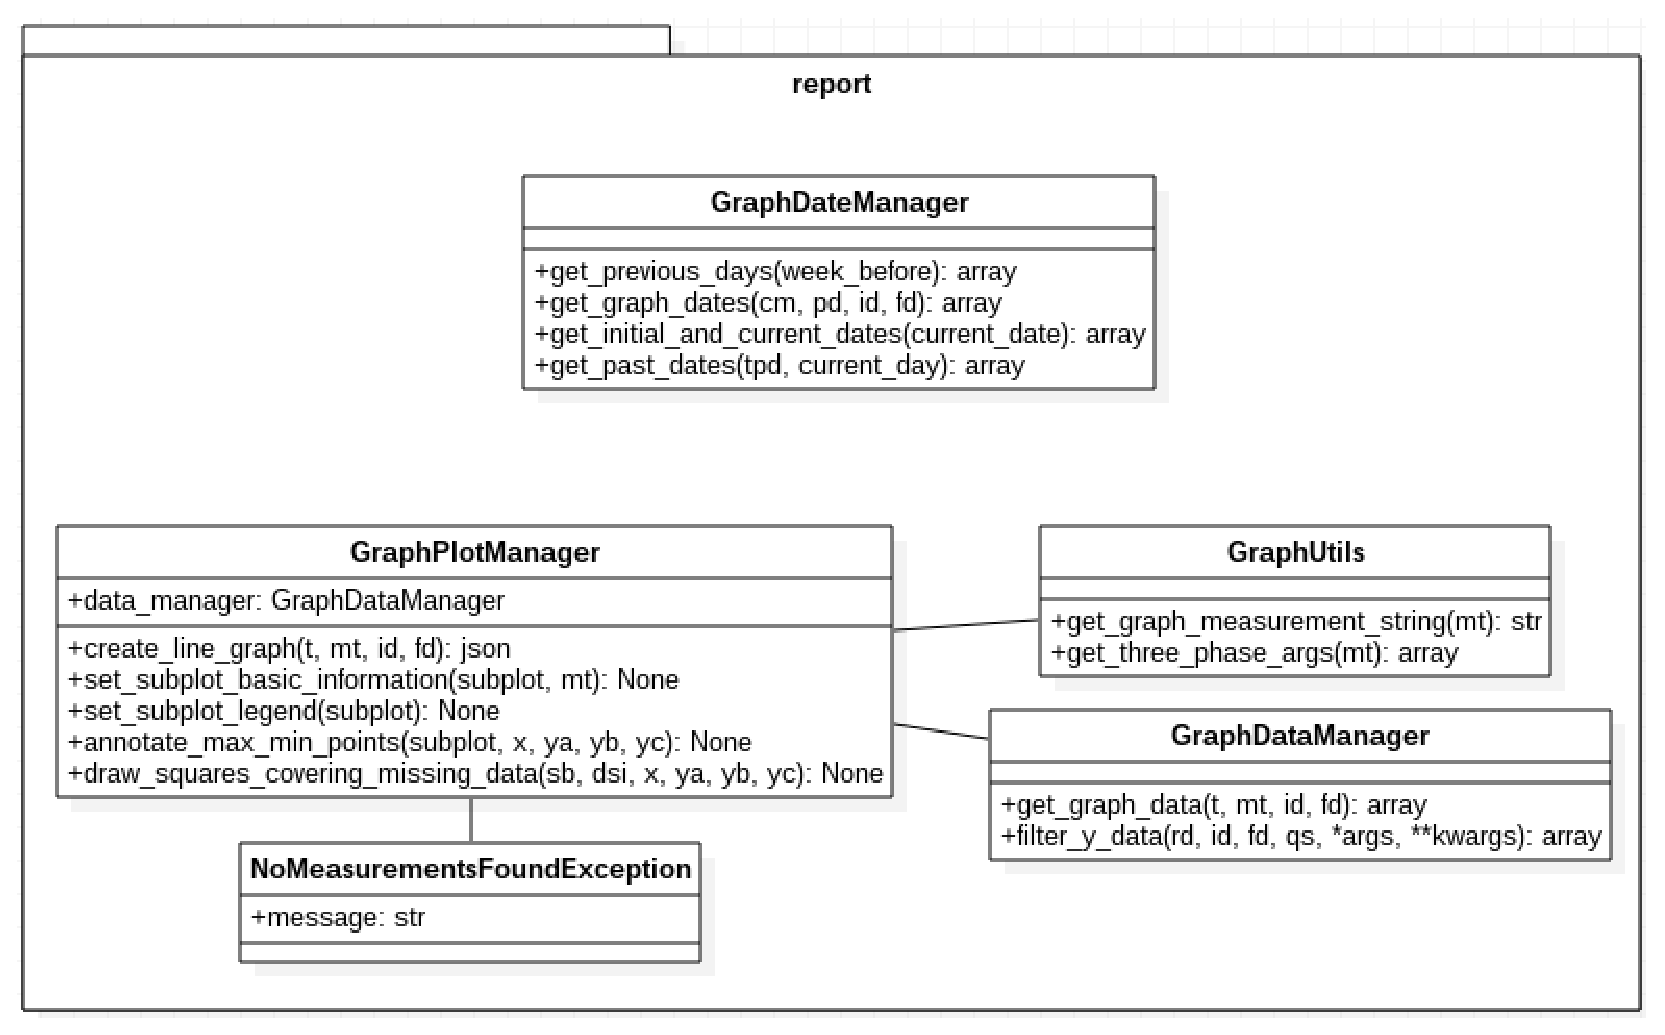
\includegraphics[keepaspectratio=true,scale=0.6]{figuras/app_report.eps}
    \caption{Diagrama de Classes para \textit{App} \textit{report}.}
    \label{app_report}
\end{figure}

Foram definidas quatro importantes classes no \textit{app} \textit{report}, sendo estas:

\begin{itemize}
    \item \textit{GraphDateManager}: realiza o tratamento e manipulação de datas, utilizadas para indicar um determinado período de medição do gráfico;
    \item \textit{GraphPlotManager}: realiza a plotagem de todos os elementos do gráfico;
    \item \textit{GraphDataManager}: realiza cálculos com os valores que serão apresentados no gráfico;
    \item \textit{GraphUtils}: indica quais serão os tipos de medições apresentados no gráfico.
\end{itemize}

Foi definido que o máximo de pontos apresentados em um gráfico seria de 200, objetivando uma geração rápida e pouca espera do usuário. Para isso, definiu-se que o período máximo para apresentação de informações seria de 1 semana e suas médias seriam realizadas da seguinte maneira:

\begin{itemize}
    \item Até 2 horas: gráfico com médias de 1 em 1 minuto;
    \item Entre 2 e 6 horas: gráfico com médias de 5 em 5 minutos;
    \item Entre 6 e 24 horas: gráfico com médias de 10 em 10 minutos;
    \item Entre 1 dia e 7 dias: gráfico com médias de 1 em 1 hora.
\end{itemize}


Para se gerar um gráfico basta selecionar um transdutor, o tipo de medição e uma opção para o período de coleta, Figura \ref{graph_options}

\begin{figure}[!h]
    \centering
    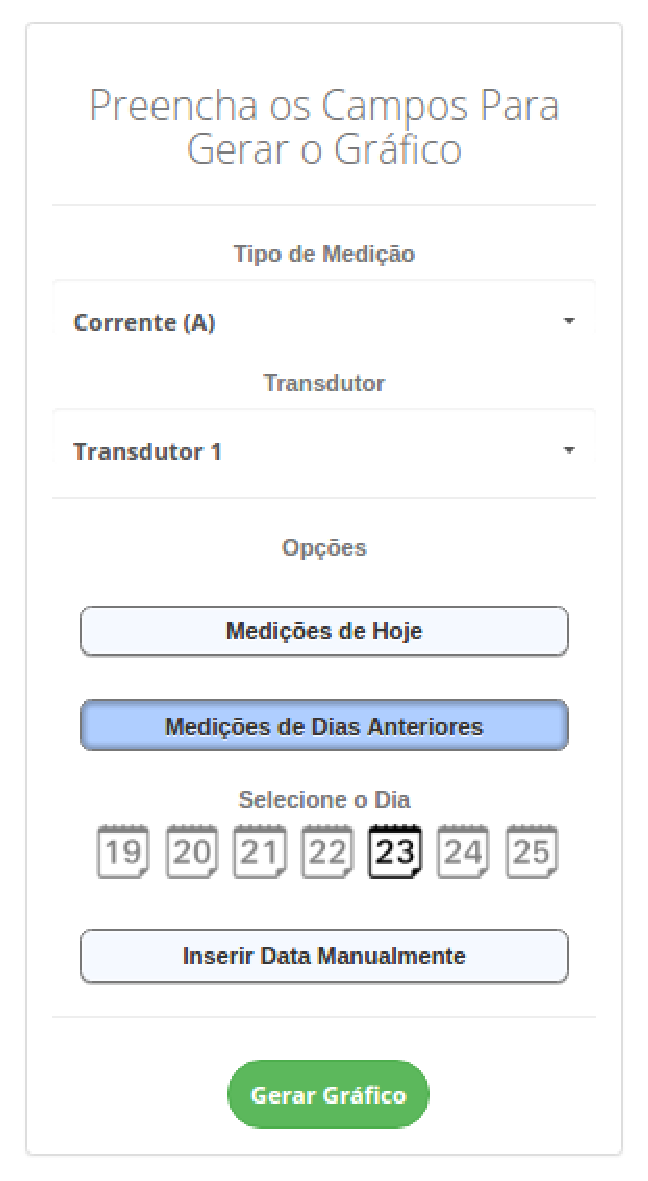
\includegraphics[keepaspectratio=true, scale=0.5]{figuras/graph_options.eps}
    \caption{Opções apresentadas para se gerar um gráfico de linhas.}
    \label{graph_options}
\end{figure}

A Figura \ref{graph_1} ilustra o gráfico de linhas com medições reais de tensão realizadas em um ambiente de teste no campus UnB-Gama, refentes ao dia 25/06/2017. É perceptível que durante a madrugada ocorrem os menores índices para tensão e os maiores durante o horário de ponta.

\begin{figure}[!h]
    \centering
    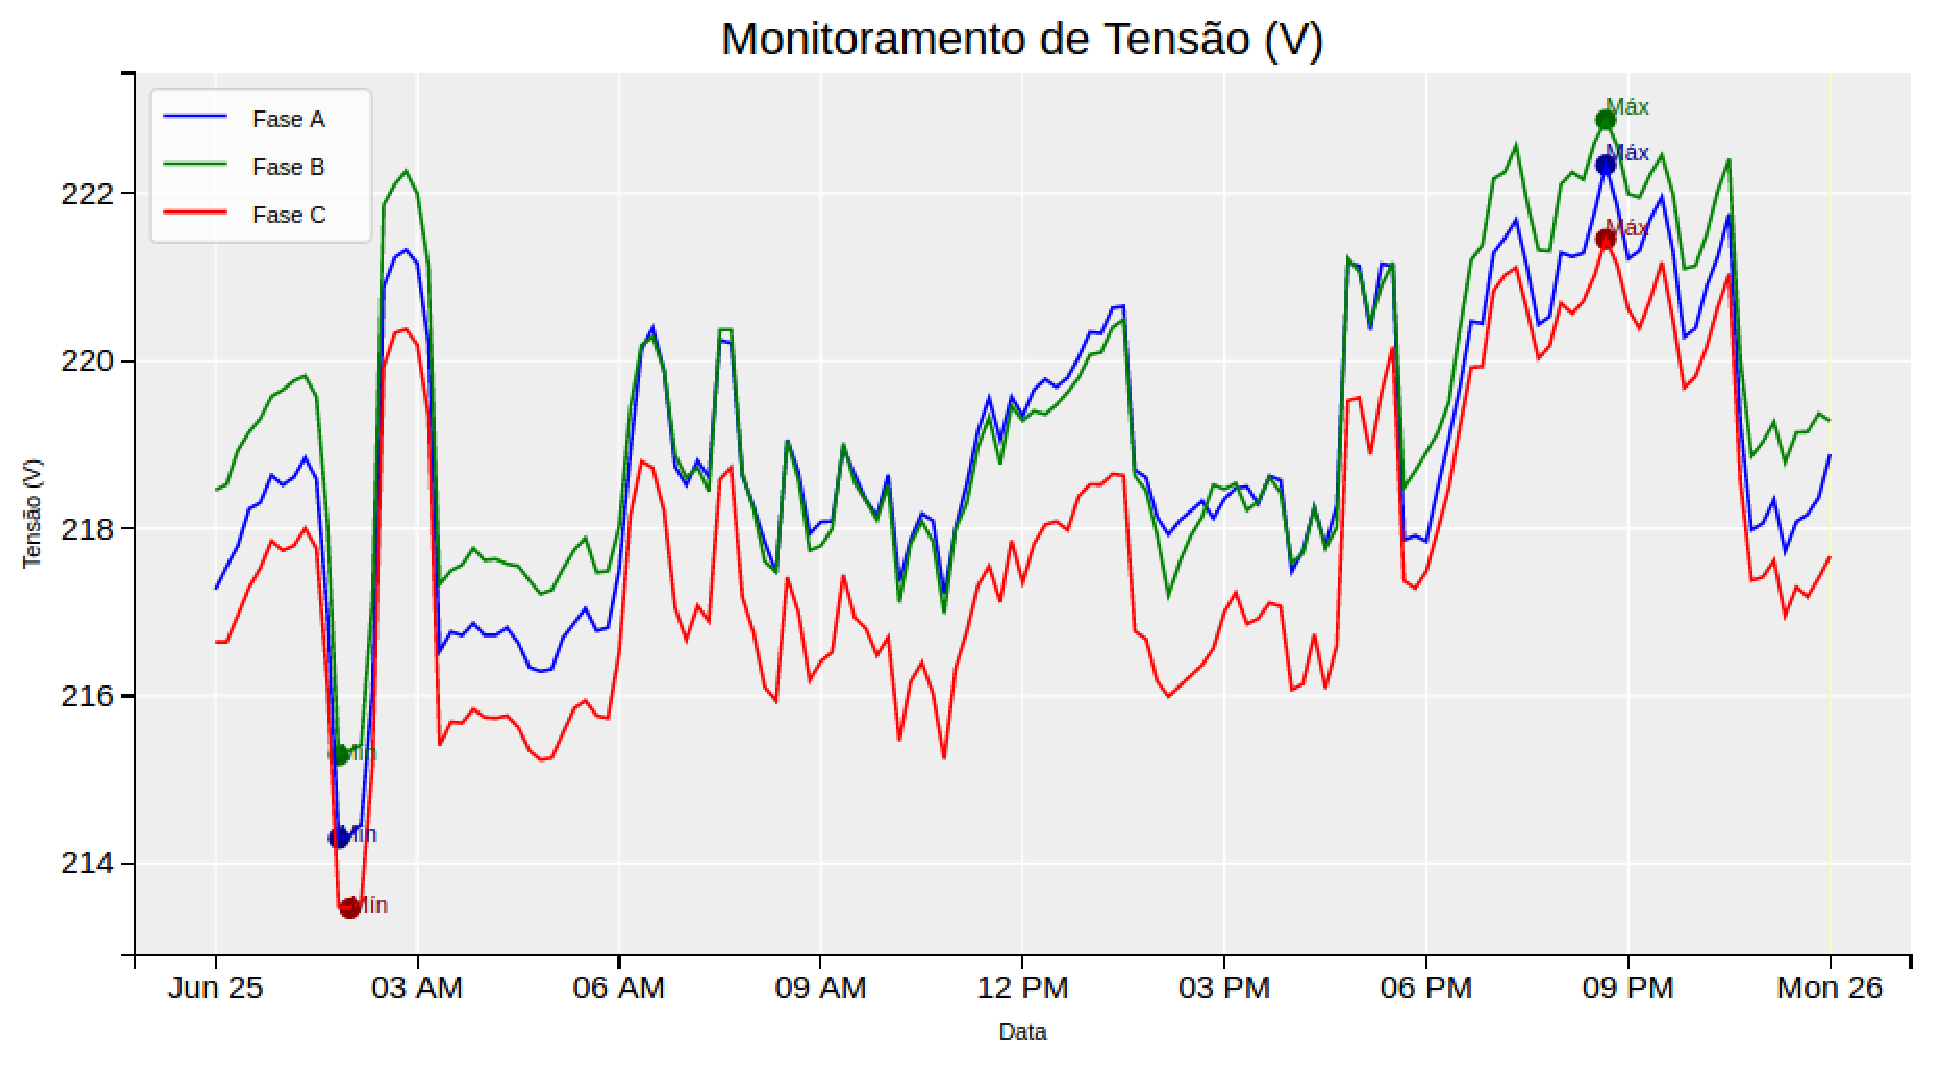
\includegraphics[keepaspectratio=true,scale=0.5]{figuras/graph_1.eps}
    \caption{Medições de tensão realizadas em ambiente de testes, referentes ao dia 25/06/2017.}
    \label{graph_1}
\end{figure}

Outro exemplo, Figura \ref{graph_2}, ilustra o gráfico de linhas gerado com medições de corrente, referentes ao dia 19/06/2017. Percebe-se nesse gráfico que houve períodos sem medições, representados pelos retângulos amarelos. Outro ponto importante a se destacar refere-se à capacidade da aplicação de continuar realizando a coleta de dados do transdutor, mesmo possuindo períodos sem realizar efetivamente uma medição.

\begin{figure}[!h]
    \centering
    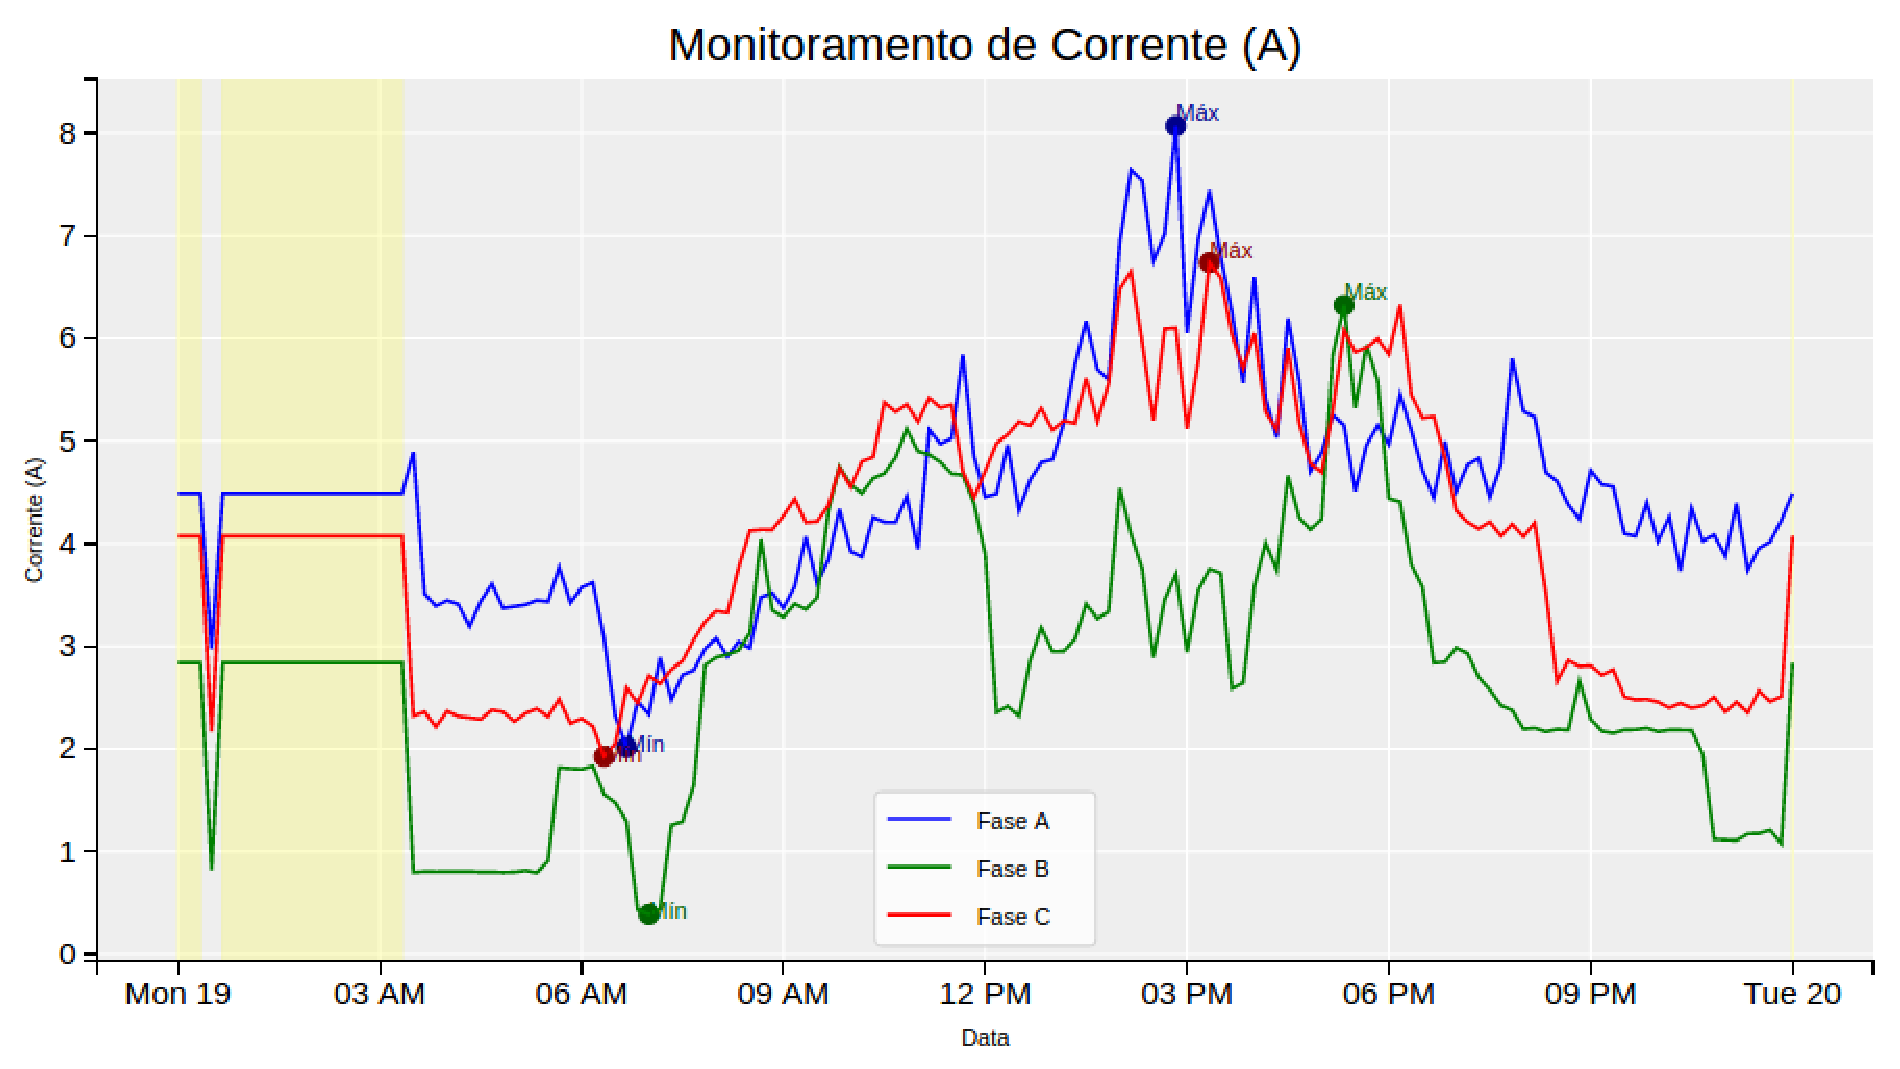
\includegraphics[keepaspectratio=true,scale=0.5]{figuras/graph_2.eps}
    \caption{Medições de corrente realizadas em ambiente de testes, referentes ao dia 19/06/2017.}
    \label{graph_2}
\end{figure}

\section{Métricas}
\subsection{\textit{SLOCCount}}
O \textit{SLOCCount}\cite{sloccount} realiza a contagem das linhas de código fonte físicas (SLOC) de um projeto. Ele determina automaticamente quais arquivos são de código-fonte suas linguagens de programação utilizadas. A ferramenta não realizada a contagem de códigos em \textit{javascript} ou HTML. Com os resultados obtidos, são apresentas estimativas de esforço, tempo de desenvolvimento, quantidade de desenvolvedores e custo. A Figura \ref{sloc} apresenta o resultado obtido pelo SMI-UnB.

\begin{figure}[!h]
    \centering
    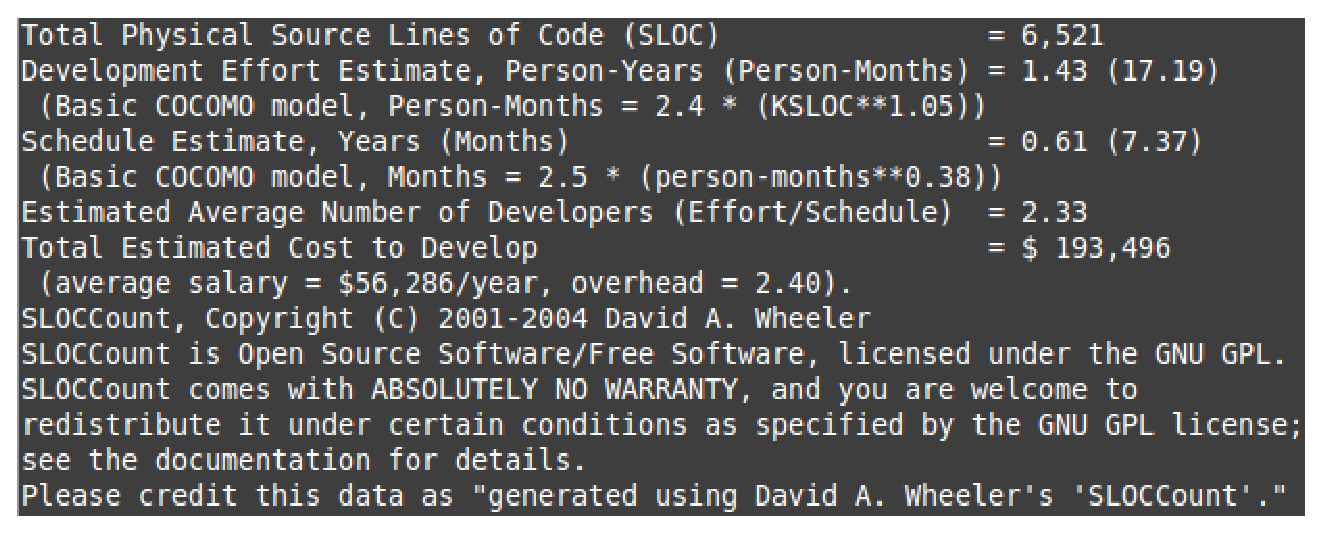
\includegraphics[keepaspectratio=true,scale=0.7]{figuras/sloc.eps}
    \caption{Análise do SMI-UnB utilizando \textit{SLOCCount}.}
    \label{sloc}
\end{figure}

Após realizada uma análise com a ferramenta, foi possível observar que o projeto teria um custo de 193,496 dólares e seria realizado em um período de aproximadamente 7 meses, com o apoio de 2 desenvolvedores. Além disso, a estimativa de tempo se aproximou ao período de 5.7 meses, refente às duas \textit{releases} do projeto.

\section{Requisitos para Utilizar o SMI-UnB}
    Para utilizar o SMI-UnB é necessário possuir, em cada servidor, uma configuração que possa executar o sistema operacional debian, sendo esta:

    \begin{itemize}
        \item Processador de 1GHz \textit{Pentium};
        \item Memória RAM de 512MB;
    \end{itemize}

    Como o projeto utiliza imagens do docker, Figura \ref{docker_size}, é necessário ter um espaço em disco de 2.6 GB, além de um espaço adicional para armazenar os registros realizados na aplicação.

    \begin{figure}[!h]
        \centering
        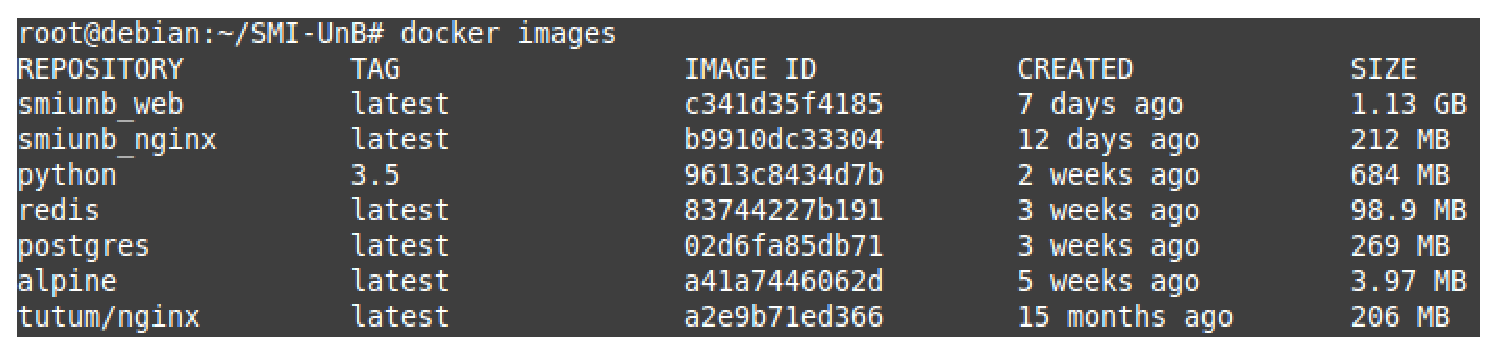
\includegraphics[keepaspectratio=true,scale=0.55]{figuras/docker_size.eps}
        \caption{Tamanho dos contêiners do Docker.}
        \label{docker_size}
    \end{figure}

    É necessária uma conexão à \textit{internet} para que seja possível realizar uma coleta de dados (protocolo UDP), sincronia de entidades (protocolo HTTP) ou prover páginas \textit{web} da aplicação.